% NICOLE CAMILLE BAIÃO - PRAXISTRANSFERBERICHT IV

% === DOKUMENTKLASSE ===
\documentclass[
    12pt, 
    a4paper,
    ]{scrartcl} % KOMA-Script-Artikelklasse mit deutscher Typografie

% === SPRACHE & ZEICHENSATZ ===
\usepackage[ngerman]{babel} % Deutsche Sprache und Silbentrennung
\usepackage{csquotes} % Typografisch korrekte Anführungszeichen

% === SEITENLAYOUT & FORMATIERUNG ===
\usepackage[a4paper, margin=2.5cm]{geometry}
\usepackage{setspace}
\setstretch{1.15}
\usepackage{fancyhdr}
\usepackage{float} % Exakte Platzierung von Gleitobjekten (z. B. Bilder)
\usepackage{caption} % Bild-/Tabellenbeschriftungen anpassen
\usepackage{adjustbox} % Elemente (z. B. Tabellen) skalieren oder ausrichten
\usepackage{makecell} % Mehrzeilige Zellen in Tabellen (Tabellen in Tabellen)
\usepackage{ragged2e}
\justifying 
% === SCHRIFTARTEN ===
\usepackage{iftex} % Prüft, ob XeTeX oder LuaTeX verwendet wird
\usepackage{fontspec} % Benutzerdefinierte Schriftarten (nur mit XeLaTeX/LuaLaTeX)
\usepackage{titlesec}
% Aktuelle Größen beibehalten:
\titleformat{\section}{\normalfont\fontsize{14}{5}\bfseries}{\thesection}{1em}{}
\titleformat{\subsection}{\normalfont\fontsize{13}{5}\bfseries}{\thesubsection}{1em}{}
\titleformat{\subsubsection}{\normalfont\fontsize{12}{5}\bfseries}{\thesubsubsection}{1em}{} 

% ABSTÄNDE ANPASSEN — Das ist der Schlüssel:
\titlespacing*{\section}{0pt}{1.1\baselineskip}{0.1\baselineskip}
\titlespacing*{\subsection}{0pt}{1.0\baselineskip}{0.1\baselineskip}
\titlespacing*{\subsubsection}{0pt}{0.9\baselineskip}{0.1\baselineskip}
 % Hauptschriftart
\setmainfont{Times New Roman} % Setzt Times New Roman als Hauptschrift

% === GRAFIKEN & ABBILDUNGEN ===
\usepackage{graphicx} % Bilder einfügen
\usepackage{xcolor} % Farben verwenden (z. B. in Code oder Text)
\usepackage{longtable}
\usepackage{tablefootnote}
% === QUELLEN & VERWEISE ===
\usepackage[
    colorlinks,       % Links ohne Umrandungen in gewählter Farbe
    linkcolor=black,  % Farbe interner Verweise
    filecolor=black,  % Farbe externer Verweise
    citecolor=black,  % Farbe von Zitaten
    urlcolor=black,    % Farbe von Links
    breaklinks
]{hyperref} % Verlinkungen
\usepackage{cleveref} % Querverweise der Querverweise
\newcommand{\etalchar}[1]{#1}

% === TABELLEN ===
\usepackage{longtable} % Tabellen über mehrere Seiten
% makecell wurde oben bereits geladen

% === CODE-DARSTELLUNG ===
\usepackage{listings} % Quellcode einfügen und formatieren

%%%%%%%%%%%%%%%%%%%%%%%%%%

% === ÜBERSCHRIFTEN-FORMATIERUNG ===
\setkomafont{sectioning}{\rmfamily\bfseries} % Überschriften fett und serifenlos

% === VERLINKUNGEN & REFERENZEN ===
\hypersetup{breaklinks=true} % Erlaubt Zeilenumbruch bei langen Links (wichtig für URLs oder Literaturverweise)
\newcommand{\anhang}[1]{\hyperref[#1]{\nameref{#1}}} % Eigener Befehl für Anhang-Verweise mit automatisch lesbarem Namen (anstatt z. B. nur "Abschnitt 5.1")

% === SEITENLAYOUT & RÄNDER ===
\geometry{
    verbose,
    tmargin=3cm,  % Oberer Rand
    bmargin=2cm,  % Unterer Rand
    lmargin=2.1cm,  % Linker Rand
    rmargin=3cm   % Rechter Rand
}

% === TYPOGRAFISCHE FEINHEITEN ===
\displaywidowpenalty = 5000
\widowpenalty=5000
\clubpenalty=5000
% === FUßNOTEN UND VERWEISE ===
\newcommand{\footfigref}[1]{\footnote{Abb. \ref{#1} auf Seite \pageref{#1}}} % Eigener Fußnotenbefehl für Bildverweise mit Seitenzahl

% === ABSTÄNDE & ABSATZFORMATIERUNG ===
\setlength{\footskip}{10mm} % Abstand zwischen Text und Fußzeile
\setlength{\abovecaptionskip}{4pt}  % Abstand oberhalb von Bild-/Tabellenunterschriften
\setlength{\belowcaptionskip}{0pt}  % Abstand unterhalb von Bild-/Tabellenunterschriften
\setlength{\intextsep}{1pc}         % Abstand bei Gleitobjekten (z. B. Bilder im Textfluss)
\setlength{\parindent}{0pt} % Kein Einzug am Absatzanfang
\setlength{\parskip}{0.75\baselineskip} % Einheitlicher Abstand zwischen Absätzen
\setstretch{1.5} % 1½-zeiliger Zeilenabstand
% === BILD- UND TABELLENUNTERSCHRIFTEN VERKLEINERN ===
\addtokomafont{caption}{\small} % Macht Bild-/Tabellenunterschriften kleiner

% === INHALTSVERZEICHNIS & LISTEN ===
\KOMAoptions{listof=entryprefix, toc=indent} % Inhaltsverzeichnis: eingerückt und mit Präfix bei Abbildungs-/Tabellenlisten

% === CODEDARSTELLUNG (SQL) ===
\lstdefinelanguage{SQL}{
    keywords={SELECT, FROM, WHERE, INSERT, INTO, VALUES, UPDATE, SET, DELETE, JOIN, LEFT, RIGHT, INNER, ORDER, BY, GROUP, ASC, DESC, CREATE, TABLE, PRIMARY, KEY, FOREIGN, ALTER, DROP, DATABASE, BEGIN, TRANSACTION, IF, EXISTS, COMMIT, AND},
    keywordstyle=\color{blue},           % Keywords blau
    comment=[l]{--},                     % Kommentare mit --
    morecomment=[s]{/*}{*/},             % Blockkommentare
    commentstyle=\color{gray},          % Kommentare grau
    stringstyle=\color{red},            % Strings rot
}

\lstset{
    basicstyle=\ttfamily\linespread{0.85}\selectfont,   % Standard-Monospace-Schrift für Listings
    keywordstyle=\bfseries\color{blue},  % Beispiel-Stil für Keywords
    commentstyle=\itshape\color{gray},   % Stil für Kommentare
    stringstyle=\color{red},            % Stil für Strings
    columns=flexible,       % Flexibler Zeilenumbruch
    language=SQL,
    breaklines=true
}

%%%%%%%%%%%%%%%%%%%%%%%%%%

% === BEGINN DOKUMENT ===
\begin{document}
% === LITERATUR EINBINDEN (alle Einträge aus der .bib ins Literaturverzeichnis) ===
\nocite{*}

% --- Seitenzahlen-Formatierung 1/3: Römische Zahlen ---
\pagenumbering{Roman}  % Nutzt römische Zahlen (I, II, III, …)
\pagestyle{fancy}      % Aktiviert fancyhdr für benutzerdefinierte Kopf-/Fußzeilen
\fancyhf{}             % Setzt alle Kopf- und Fußzeilen zurück
\fancyhead[R]{\thepage}  % Seitenzahl oben rechts anzeigen
\renewcommand{\headrulewidth}{0pt} % Keine Linie in der Kopfzeile
\renewcommand{\footrulewidth}{0pt} % Keine Linie in der Fußzeile

%%%%%%%%%%%%%%%%%%%%%%%%%%

% === BEGINN TITELSEITE ===
\begin{titlepage}
\begingroup
\setstretch{1.15} % Nur auf der Titelseite engerer Zeilenabstand
\centering % Zentriert den gesamten Inhalt der Titelseite
   
% --- Logos einfügen (links und rechts) ---

\includegraphics[scale=0.15]{BILDER-PTB4/Berliner-wasserbetriebe.svg.png}\hfill % \hfill sorgt dafür, dass die beiden Logos links und rechts stehen

\includegraphics[scale=0.25]{BILDER-PTB4/Hochschule_für_Wirtschaft_und_Recht_Berlin_logo.jpg} \\[1.0cm] % \\[1.8cm] fügt einen vertikalen Abstand von 1.8 cm nach den Bildern ein

% --- Titel (fette und große Schrift) ---
\Large{\textbf{Projektcontrolling bei agilen IT-Einführungsprojekt am Beispiel der Einführung von SAP SucessFactors Learning}} \\[0.8cm]

% --- Untertitel ---
{\Large Studienarbeit (Hausarbeit)} \\

% --- Neuer Text mit Abstand --
\vspace{0.8cm} % Abstand zum Unterschift
\large % Setzt die Schriftgröße auf Standard
vorgelegt am 17.08.2026 an der\\ [0.2cm]
Hochschule für Wirtschaft und Recht Berlin\\ [0.2cm]
Fachbereich Duales Studium\\ [0.4cm]
\vspace{0.8cm} % Abstand zur Tabelle

% --- Tabelle mit persönlichen Angaben ---
{\large
\begin{tabular}{l l}  
    \textbf{von:} & Nicole Camille Baião  \\[0.1cm]
    \textbf{Bereich:} & Wirtschaft \\[0.1cm]
    \textbf{Fachrichtung:} & Wirtschaftsinformatik \\[0.1cm]
    \textbf{Studienjahrgang:} & 2024 \\[0.1cm]
    \textbf{Studienhalbjahr:} & 4. Semester \\[0.1cm]
    \textbf{Ausbildungsbetrieb:} & Berliner Wasserbetriebe  \\[0.1cm]
    \textbf{Betreuender Prüfer:} & Prof. Dr. Olaf Resch \\[0.1cm]
    \textbf{Betreuer im Betrieb:} & Michael Schneider \\[0.7cm]
\end{tabular}
}

% --- Bereich für Unterschriften ---
\raggedright % Setzt den folgenden Text linksbündig
\textbf{\normalsize{Vom Ausbildungsleiter zur Kenntnis genommen:}} \\[1.0cm]

% --- Tabelle mit Unterschriften ---
\begin{tabular}{p{8cm} p{8cm}}
    \normalsize{Berlin, den 07. August 2026} & \normalsize{Berlin, den 07. August 2026} \\[0.03cm]

    
\includegraphics[width=5.7cm]{BILDER-PTB4/unterschrift_nicole.png} &
    \raisebox{-0.25cm}{
\includegraphics[width=5cm]{BILDER-PTB4/michael.png}} \\[-0.25cm]

    \normalsize{\underline{\hspace{5.5cm}}} & \normalsize{\underline{\hspace{5.5cm}}} \\[0.1cm]
    \normalsize{(Unterschrift der Studentin)} & \normalsize{(Unterschrift des Ausbildungsleiters)}
\end{tabular}
% === ENDE TITELSEITE ===
\endgroup
\end{titlepage}

% === Inhaltsverzeichnis === 
\setcounter{page}{1} % Setzt die Seitennummer auf 1 für neue Zählung (Neustart der Zählung)
\newpage
\section*{Inhaltsverzeichnis}  
\renewcommand{\contentsname}{}
\vspace{-1.3cm}  % Anpassung des vertikalen Abstands
\tableofcontents % Inhaltsverzeichnis erstellen

% === Abkürzungsverzeichnis === 
\newpage
\section*{Abkürzungsverzeichnis}  
\addcontentsline{toc}{section}{Abkürzungsverzeichnis}
\vspace{0.6cm}
\begin{tabular}{p{4cm} p{11.35cm}}   
    \textbf{\normalsize BWB:} & \normalsize Berliner Wasserbetriebe \\[0.5cm]
    \hline
    \textbf{\normalsize DIN:} & \normalsize Deutsches Institut für Normung \\[0.5cm]
    \hline
    \textbf{\normalsize IT-Z/P:} & \normalsize IT-Zentrale Aufgaben - Projekte \\[0.5cm]
    \hline
    \textbf{\normalsize SAP:} & \normalsize Systeme, Anwendungen und Produkte in der Datenverarbeitung \\[0.5cm]
 \end{tabular}

% --- Seitenzahlen-Formatierung 2/3: Wechsel auf normale (arabische) Zahlen ---
\newpage
\pagenumbering{arabic} % Normale Zahlen ab "Einleitung"
\setcounter{page}{1}

% === Einleitung ===

\section{Einleitung}

\subsection{Problemstellung und Relevanz des Themas}
Die fortschreitende Digitalisierung verändert die Art und Weise, wie Unternehmen ihre internen Prozesse organisieren. Insbesondere im Personalwesen werden zunehmend cloudbasierte Standardlösungen eingeführt, um historisch gewachsene Einzelsysteme abzulösen und den Pflegeaufwand zu senken. Die Einführung einer neuen Softwarelösung ist dabei kein rein technischer Vorgang, sondern ein komplexes Projekt, das fachliche, organisatorische und rechtliche Anforderungen miteinander verbinden muss.

IT-Einführungsprojekte gelten als anspruchsvoll und ressourcenintensiv; ein erheblicher Anteil dieser Vorhaben verfehlt die ursprünglich gesetzten Ziele hinsichtlich Zeit, Budget oder Qualität. Eine wesentliche Ursache liegt darin, dass sich die Anforderungen an das System im Projektverlauf häufig verändern. Um auf solche Änderungen flexibel reagieren zu können, gewinnen agile und iterative Vorgehensweisen gegenüber rein klassischen, plangetriebenen Ansätzen an Bedeutung.

Hieraus ergibt sich ein Spannungsfeld für das Projektcontrolling: Das klassische Controlling steuert ein Projekt über fest definierte Zeit-, Budget- und Meilensteinpläne und orientiert sich am sogenannten magischen Dreieck aus Zeit, Kosten und Leistungsumfang. In einem agilen Umfeld, in dem sich der Leistungsumfang laufend weiterentwickelt, lassen sich diese Instrumente jedoch nicht ohne Weiteres anwenden. Es stellt sich daher die Frage, wie ein Projektcontrolling gestaltet sein muss, das einerseits die notwendige Transparenz über Fortschritt, Kosten und Risiken sicherstellt und andererseits der Dynamik agiler IT-Einführungsprojekte gerecht wird.

Die praktische Relevanz zeigt sich am Beispiel der Berliner Wasserbetriebe, die ihr abgekündigtes Lernmanagementsystem durch das cloudbasierte Modul SAP SuccessFactors Learning ablösen. Da über dieses System unter anderem gesetzlich vorgeschriebene Pflicht- und Sicherheitsschulungen revisionssicher verwaltet werden müssen und zahlreiche Bereiche, Standorte und Personengruppen betroffen sind, ist eine verlässliche Steuerung des Einführungsprojektes von hoher Bedeutung. Das Projekt bietet damit ein geeignetes Praxisbeispiel, um die Konzeption und Umsetzung eines Projektcontrollings bei einer IT-Systemeinführung zu untersuchen.

\subsection{Zielsetzung und Forschungsfrage}
Ziel der vorliegenden Arbeit ist es, ein Projektcontrolling für die Einführung einer IT-Standardsoftware methodisch zu konzipieren und seine Umsetzung anhand eines konkreten Praxisbeispiels zu untersuchen. Im Mittelpunkt steht die Frage, welche Controlling-Instrumente und Kennzahlen geeignet sind, um ein agil bzw. iterativ durchgeführtes Einführungsprojekt wirksam zu steuern. Daraus leitet sich die folgende zentrale Forschungsfrage ab:

\textit{„Wie kann Projektcontrolling im Rahmen einer agilen IT-Systemeinführung methodisch konzipiert und in der Praxis umgesetzt werden?“}

Zur Beantwortung dieser übergeordneten Frage werden folgende Teilfragen betrachtet: Welche Aufgaben und Instrumente umfasst das Projektcontrolling im klassischen und im agilen Kontext? Wie lassen sich klassische und agile Steuerungselemente sinnvoll miteinander verbinden? Und welche praktischen Handlungsempfehlungen ergeben sich aus dem Praxisbeispiel für vergleichbare IT-Einführungsprojekte? Die Arbeit verfolgt damit nicht allein ein theoretisches, sondern ausdrücklich ein anwendungsorientiertes Ziel und mündet in konkrete Handlungsempfehlungen.

\subsection{Methodisches Vorgehen und Aufbau der Arbeit}
Methodisch verbindet die Arbeit eine Literaturrecherche mit einer Praxisanalyse. Die theoretischen Grundlagen zum Projektmanagement und insbesondere zum Projektcontrolling werden auf Basis wissenschaftlicher Literatur erarbeitet. Die Arbeit folgt dabei einem induktiven Ansatz: Ausgehend vom konkreten Einzelfall werden übertragbare Erkenntnisse für die Steuerung agiler IT-Einführungsprojekte abgeleitet. Als Datengrundlage dienen neben der wissenschaftlichen Literatur interne Projektunterlagen der Berliner Wasserbetriebe.

Nach der Einleitung stellt Kapitel 2 die Grundlagen des Projektcontrollings dar, bevor Kapitel 3 das methodische Vorgehen und das Praxisprojekt vorstellt und Kapitel 4 das Controlling daran analysiert. Kapitel 5 reflektiert die Ergebnisse kritisch mit Handlungsempfehlungen, Kapitel 6 fasst zusammen, beantwortet die Forschungsfrage und gibt einen Ausblick. 

\section{Theoretische Grundlagen des Projektscontrollings}

\subsection{Begriff und Ziele des Projektsmanagements}
Ein Projekt ist nach DIN 69901 „ein Vorhaben, das im Wesentlichen durch die Einmaligkeit der Bedingungen in ihrer Gesamtheit gekennzeichnet ist",\footnote{\cite{Feidler_ControllingVonProjekten}, S.~2.} also keine Routineaufgabe, sondern zeitlich begrenzt, mit beschränkten Ressourcen und festgelegtem Ziel.\footnote{Vgl. \cite{Feidler_ControllingVonProjekten}, S.~2-3.} Das Projektmanagement umfasst die Führungsaufgaben für Initiierung, Definition, Planung, Steuerung und Abschluss von Projekten. Seine Ziele werden im „magischen Dreieck" aus Sachzielen (Leistung/Qualität), Terminzielen und Kostenzielen zusammengefasst, die sich gegenseitig beeinflussen.\footnote{Vgl. \cite{Feidler_ControllingVonProjekten}, S.~5-6.}

Grundsätzlich lassen sich zwei Arten des Projektmanagements unterscheiden: Das klassische (traditionelle) Projektmanagement zerlegt ein Projekt in Projektphasen, definiert zu Meilensteine (Etappenziele) und arbeitet dann Phase für Phase ab; die Projektziele werden zu Beginn festgelegt, danach wird geplant, umgesetzt und am Ende das fertige Produkt dem Kunden übergeben. Das agile Projektmanagement durchläuft das Projekt eine Vielzahl kleiner, sich wiederholender Schritte („Iterationen"), an deren Ende jeweils ein weiterentwickeltes Zwischenergebnis steht, zu dem der Kunde ein Feedback abgibt, bevor die nächste Iteration beginnt. Auf diesen beiden Vorgehensweisen bauen das klassische Projektcontrolling und das Controlling in agilen Projekten auf.\footnote{Vgl. \cite{Beiderwieden_ProjektmanagementIT}, S.~11.}

\subsection{Controlling in klassischen Projekten}
Das Controlling unterstützt die Unternehmensführung bei Planung und Kontrolle und versorgt das Management mit entscheidungsrelevanten Informationen.\footnote{Vgl. \cite{Feidler_ControllingVonProjekten}, S.~8.} Darauf aufbauend beschreibt die DIN 69901 das Projektcontrolling als Regelkreis zur „Sicherung des Erreichens der Projektziele durch: Soll-Ist-Vergleich, Feststellung der Abweichungen, Bewerten der Konsequenzen und Vorschlagen von Korrekturmaßnahmen, Mitwirkung bei der Maßnahmenplanung und Kontrolle der Durchführung".\footnote{\cite{Feidler_ControllingVonProjekten}, S.~8} Sein zentrale Ziel besteht somit darin, das Erreichen der Projektziele abzusichern, nicht beschränkt auf Kosten, sondern mit umfassendem Servicecharakter.\footnote{Vgl. \cite{Feidler_ControllingVonProjekten}, S.~10.} Damit unterstützt es das Projektmanagement bei der Abstimmung der strategischen und operativen Projektmanagementaufgaben, insbesondere bei der Projektplanung und -kontrolle, und sichert dessen Rationalität.\footnote{Vgl. \cite{Feidler_ControllingVonProjekten}, S.~11.} Die Verantwortung ist klar verteilt: Der Projektleiter verantwortet das Ergebnis, Leistung und Termine, der Projektcontroller vor allem die Transparenz der Daten.\footnote{Vgl. \cite{Feidler_ControllingVonProjekten}, S.~15.}

Bei klassisch (plangetrieben) abgewickelten Projekten steht die Einhaltung von Zeit- und Kostenvorgaben im Vordergrund, da Zeitverzögerungen in einem Projektabschnitt häufig auf nachfolgende Arbeitsschritte durchschlagen und meist höhere Kosten verursachen.\footnote{Vgl. \cite{Nobach_Projektcontrolling}, S.61.} Zur laufenden Steuerung nachfolgend die Meilenstein-Trendanalyse für das Termin- und Kostencontrolling sowie die Risikomatrix für das Risikocontrolling.

\subsubsection{Termin- und Kostencontrolling}
Für ein zeitliches Kontrollsystem wird das gesamte Projekt in kleinere, möglichst gleich große Zeitabschnitte eingeteilt von höhestens etwas vier Wochen unterteilt, deren Abschluss jeweils mit einem Meilensteinen - einem überprüfbaren, vordefinierten Ergebnis mit festem Termin und definierten Kosten - markiert wird.\footnote{Vgl. \cite{Nobach_Projektcontrolling}, S~62.}

Zur Überwachung der Meilensteinerreichung eignet sich vor allem die Meilenstein-Trendanalyse, da sie den Projektfortschritt im Zeitablauf nachhält und – anders als ein einfaches Balkendiagramm – frühzeitig aufzeigt, ob sich Zeitverzögerungen anbahnen.\footnote{Vgl. \cite{Nobach_Projektcontrolling}, S.62.} Im Meilenstein-Trenddiagramm zeigt die horizontale Achse den Berichtszeitpunkt und die vertikale den erwarteten Fertigstellungstermin des Meilensteins; durch die symmetrische Darstellung entsteht eine Verbindungslinie im 45°-Winkel.\footnote{Vgl. \cite{Nobach_Projektcontrolling}, S~63-64.}
Der Kurvenverlauf lässt sich wie folgt interpretieren:
\begin{itemize}
    \setlength\itemsep{0.4\baselineskip}
    \setlength\parskip{0pt}
    \setlength\parsep{0pt}
    \item \textbf{Auswärtsbewegung} (oberhalb der Ursprungslinie): terminliche Verzögerung, der geplante Endtermin ist voraussichtlich nicht einzuhalten (terminkritisch).
    \item \textbf{Abwärtsbewegung:} der Meilenstein wird voraussuchtlich vor dem geplanten Termin erreicht.
    \item \textbf{horizontale Linie:} der ursprünglich geplante Fertigstellungstermin wurde in jedem bisherigen Berichtszeitpunkt bestätigt.\footnote{Vgl. \hyperref[sec:Anhang1]{Anhang 1}}
\end{itemize}
Dieselbe Grundmethodik lässt sich über Kosten-Trenddiagramme auf die Entwicklung der prognostizierten Gesamtkosten übertragen. Da beide Analysen durch Verdichtung nur Indizien liefern, sollten sie mit einem Frühwarnsystem kombiert und den Fertigstellungsgrad ergänzt werden.\footnote{Vgl. \cite{Nobach_Projektcontrolling}, S~65.}

\subsubsection{Leistungs- und Qualitätscontrolling}
Eine zentrale Schwierigkeit liegt in der zuverlässigen Ermittlung des Leistungsfortschritts. Befragt man die verantwortlichen Mitarbeiter, besteht die Gefahr, dass der Fertigstellungsgrad zu hoch eingeschätzt wird („Fast-schon-fertig-Syndrom"): Bis kurz vor Projektende wird angenommen, die geplante Leistung noch erfüllen zu können, obwohl bereits eine nicht mehr auszugleichende Planabweichung vorliegt. Verstärkt wird dies durch Qualitätsmängel, die oft erst spät entdeckt werden und Nacharbeiten auslösen; je geringer die Qualität und je später Mängel auffallen, desto größer wird die Lücke zwischen angenommenem und tatsächlichem Leistungsfortschritt.\footnote{Vgl. \cite{Feidler_ControllingVonProjekten}, S~133-134.}
Zur objektiveren Bestimmung des Leistungsfortschritts stehen mehrere Methoden zur Verfügung.\footnote{Vgl. \cite{Feidler_ControllingVonProjekten}, S~136.}
\begin{itemize}
    \setlength\itemsep{0.4\baselineskip}
    \setlength\parskip{0pt}
    \setlength\parsep{0pt}
    \item \textbf{Meilenstein-Methode:} Verhältnis der erreichten zu allen geplanten Meilensteinen; setzt voraus, dass genügend differenzierte Meilensteine vorliegen.
    \item \textbf{0/50/100-Methode:} Noch nicht begonnene Arbeitspakete werden mit 0\,\%, begonnene mit 50\,\% und abgeschlossene mit 100\,\% bewertet; der Fehler der undifferenzierten 50\,\%-Zuordnung gleicht sich über viele Arbeitspakete meist aus.
    \item \textbf{Efforts-Expended-Methode:} Ist-Aufwand geteilt durch den voraussichtlichen Gesamtaufwand (Ist-Aufwand plus realistisch geschätzter Restaufwand).
\end{itemize}

\subsection{Controlling in agilen Projekten}
Beim agilen Ansatz ist zu berücksichtigen, dass anders als beim klassischen (deterministischen) Termin- und Ressourcencontrolling kein Basisplan als Referenz zur Fortschrittskontrolle herangezogen werden kann, da aufgrund des iterativen Vorgehens jederzeit mit Anforderungsänderungen zu rechnen ist und ein ursprünglicher Basisplan somit zu jedem Zeitpunkt hinfällig wäre.\footnote{Vgl. \cite{Mayrhofer_HybridesProjektmanagement}, S.~114.} Das agile Controlling setzt deshalb an der Vorgehensweise von Scrum an: Scrum-Projekte bestehen aus einer Abfolge kurzer Iterationen, den Sprints (maximal 30 Tage), an deren Ende jeweils ein auslieferbares Produktinkrement steht; die Anforderungen werden als User Stories mit Story Points geschätzt.\footnote{Vgl. \cite{Beiderwieden_ProjektmanagementIT}, S.~114.} Aus diesen Größen leitet das Controlling seine Instrumente für Termine, Kosten und Qualität ab.

\subsubsection{Termin- und Kostencontrolling}
Das zentrale Instrument der Terminüberwachung im Scrum ist das Burndown-Chart. Dazu werden die noch verbleibenden Aufgaben bzw. offenen Story Points in regelmäßigen Abständen gezählt täglich im Daily Scrum oder jeweils zum Sprint-Ende und über den zeitlichen Verlauf (Sprint-Tage) abgetragen. Das Diagramm stellt zwei Linien gegenüber: den prognostizierten Idealverlauf der offenen Aufgaben, der gleichmäßig auf null zuläuft, und den tatsächlichen Verlauf. Aus der Lage der Ist-Linie zum Idealverlauf lässt sich der Terminstand ablesen: Liegt der tatsächliche Verlauf oberhalb des Idealverlaufs, wurden die Aufgaben langsamer als geplant abgearbeitet und es besteht ein Rückstand; liegt er unterhalb, wurden mehr Aufgaben als geplant erledigt und es besteht ein Vorsprung.\footnote{Vgl. \cite{Mayrhofer_HybridesProjektmanagement}, S.~115.}

Die Steigung der Kurve repräsentiert die relative Effizienz des Teams, die sogenannte Velocity. Ein flacherer Verlauf im Vergleich zum Idealverlauf zeigt eine niedrigere Velocity als geplant an, ein steilerer Verlauf eine höhere. Weicht die Velocity ab, kann situationsbedingt gegengesteuert werden etwa durch Anpassung des Sprint-Plans, durch Grooming (Überarbeitung) des Product Backlog oder durch Reduktion bzw. Erhöhung der pro Sprint geplanten Story Points. Dabei ist der Lerneffekt des Teams zu berücksichtigen, da eine anfangs niedrige Velocity in den ersten Sprints in den Folge-Sprints zunehmen kann. Analog lässt sich auf gleiche Weise ein Burnup-Chart einsetzen, das statt der verbleibenden die kumuliert erledigten Aufgaben abbildet.\footnote{Vgl. \hyperref[sec:Anhang3]{Anhang 3}}

Für das Kostencontrolling agiler Projekte kann die Earned-Value-Analyse (EVA) eingesetzt werden.
Bei ihrer Anwendung ist allerdings zu berücksichtigen, dass wegen möglicher Anforderungsänderungen im Projektverlauf anders als bei deterministischen Projekten größere Unsicherheiten in Bezug auf die Prognosen bestehen. Die Earned-Value-Analyse verbindet die Kostenbetrachtung mit dem tatsächlich erreichten Arbeitsfortschritt und stützt sich dabei im Wesentlichen auf drei Größen: die Ist-Kosten der abgeschlossenen Arbeit (IKAA), die Soll-Kosten der abgeschlossenen Arbeit bzw. den Earned Value (SKAA) sowie die Plan-Kosten (PK).\footnote{Vgl. \cite{Mayrhofer_HybridesProjektmanagement}, S.~124-125.}

Aus dem Vergleich dieser Größen lassen sich Abweichungen und Prognosen ableiten, insbesondere die Kostenabweichung (KA) als Differenz zwischen Soll- und Ist-Kosten der abgeschlossenen Arbeit, die voraussichtlichenberechneten Kosten bei Projektende (BK) sowie ein Kostenleistungsindex (KLI) als Verhältnis von erbrachter Leistung zu den dafür angefallenen Ist-Kosten. Auf diese Weise wird sichtbar, ob und in welchem Umfang die Ist-Kosten die Soll-Kosten der abgeschlossenen Arbeit übersteigen, also eine Budgetüberschreitung vorliegt.\footnote{Vgl. \cite{Mayrhofer_HybridesProjektmanagement}, S.~124-125.} Da die Analyse den Fertigstellungsgrad einbezieht, verknüpft sie das Kostencontrolling unmittelbar mit dem tatsächlichen Leistungsfortschritt und liefert so eine belastbarere Aussage als eine reine Gegenüberstellung von Plan- und Ist-Kosten.\footnote{Vgl. \hyperref[sec:Anhang4]{Anhang 4}}

\subsubsection{Leistungs- und Qualitätscontrolling}
Für das Qualitätscontrolling dient im agilen Vorgehen die Definition of Done als zentraler Maßstab. In ihr vereinbart das Scrum-Team vorab alle Qualitätsmerkmale, die erfüllt sein müssen, damit eine User Story als abgeschlossen gilt.\footnote{Vgl. \cite{Beiderwieden_ProjektmanagementIT}, S.~117.} Sie legt damit anhand konkreter, überprüfbarer Kriterien fest, wann eine Anforderung tatsächlich erfüllt ist, und schafft ein einheitliches Qualitätsverständnis im Team; zugleich stellt sie sicher, dass zum vereinbarten Termin (Timeboxing) die Aufgabe vollumfänglich, aber auch nicht über das Notwendige hinaus erledigt wird.\footnote{Vgl. \cite{Lang_Schops_Praxisleitfaden}, S.~90.}

Die eigentliche Qualitätskontrolle erfolgt am Ende jedes Sprints im Sprint Review: Dort wird das entwickelte Sprintergebnis vorgeführt und daran gemessen, was laut Definition of Done als fertiggestellt gilt. Teilnehmer sind der Scrum Master, das Entwicklungsteam, der Product Owner und die eingeladenen Stakeholder, insbesondere der Kunde, der Rückmeldung zum Zwischenergebnis gibt.\footnote{Vgl. \cite{Beiderwieden_ProjektmanagementIT}, S.~117.} Für das Controlling ist dieser Maßstab entscheidend, weil eine Aufgabe erst dann als „fertig" in die Termin- und Kostenkennzahlen eingeht, wenn sie die vereinbarten Qualitätskriterien erfüllt. Dadurch wird verhindert, dass ein zu optimistisch gemeldeter Fertigstellungsgrad das Burndown-Chart oder die Earned-Value-Analyse verzerrt.

\subsection{Risikocontrolling}
Ein weiteres zentrales Instrument des klassischen Projektcontrollings ist die Risikomatrix. Sie dient dazu, identifizierte Projektrisiken nach Eintrittswahrscheinlichkeit und Auswirkung einzustufen. Der zugehörige Risikofaktor ergibt sich aus der Eintrittswahrscheinlichkeit multipliziert mit der Auswirkung und kann Werte zwischen 0 (keine Auswirkung) und 1 (extreme Auswirkung) annehmen. Mithilfe eines Ampelsystems werden die Risiken anhand des Risikofaktors in drei Kategorien eingeteilt:\footnote{Vgl. \cite{Nobach_Projektcontrolling}, S.~88.}
\begin{itemize}
    \setlength\itemsep{0.4\baselineskip}
    \setlength\parskip{0pt}
    \setlength\parsep{0pt}
    \item \textbf{grün (0–0,2):} kein bzw. minimales Risiko ohne wesentliche Auswirkungen; Gegenmaßnahmen sind nicht zwingend notwendig.
    \item \textbf{gelb (0,2–0,5):} mittleres Risiko; keine existenzbedrohende Gefährdung, es sollten aber Gegenmaßnahmen ergriffen werden.
    \item \textbf{rot (0,5-1):} hohes Risiko, das bei Eintritt den gesamten Projekterfolg gefährden kann.\footnote{Vgl. \hyperref[sec:Anhang2]{Anhang 2}}
\end{itemize}
Das Ampelsystem dient als visuelles Frühwarnsystem, das den aktuellen Risikostatus eines Projekts auf einen Blick verdeutlich. Durch die farbliche Kennzeichnung können Handlungsbedarf und Prioritäten schnell erkannt sowie Entscheidungen im Projektcontrolling und Reporting erleichtert werden.\footnote{Vgl. \cite{Factro_Ampelstatus}} Die wichtigsten (Top-)Risiken lassen sich zudem in einer Risk Map darstellen und regelmäßig im Projektlenkungsausschuss berichten.\footnote{Vgl. \cite{Nobach_Projektcontrolling}, S.~90.}

\section{Vorstellung des Praxisprojekts}

\subsection{Ausgangssituation bei den Berliner Wasserbetrieben}

Ausgangspunkt des Projekts ist die Abkündigung der bisherigen Lösung IMC Learning Suite (intern AQUA.learn genannt) durch den Hersteller, sodass eine neue Software zwingend benötigt wird. Angestrebt wird eine cloudbasierte Standardanwendung, die sich in die bereits genutzte SuccessFactors-Landschaft (Recruiting sowie Performance \& Goals) einfügt und der strategischen IT-Vorgabe folgt, die Anzahl der eingesetzten Anwendungen zu reduzieren.\footnote{Vgl. \hyperref[sec:Anhang5]{Anhang 5}, Frage~1. und Frage~6.} Da über das System künftig unter anderem gesetzlich vorgeschriebene Pflicht- und Sicherheitsschulungen revisionssicher verwaltet werden müssen, ist eine verlässliche Steuerung des Einführungsprojekts von hoher Bedeutung.\footnote{Vgl. \hyperref[sec:Anhang5]{Anhang 5}, Frage~1 und Frage~9.}

\subsection{Projektphasen und hybrides Vorgehen}

Voraussetzung für den Projektstart bei den BWB ist die Freigabe eines Projektauftrags, in dem Ziele und Anforderungen durch den Auftraggeber -- das Personalmanagement (PM) bzw. die Personalentwicklung -- schriftlich dokumentiert werden.\footnote{Vgl. \hyperref[sec:Anhang5]{Anhang 5}, Frage~17.}

Der weitere Ablauf folgt einem hybriden Vorgehen aus klassischem, phasenorientiertem Projektmanagement mit definierten Freigabepunkten (Projektauftrag, Umsetzungskonzept, Zustimmung zur Produktivsetzung, Projektabschluss) und agiler, iterativer Realisierung in mehreren Iterationen mit jeweils abschließendem Test- und Freigabezyklus (Kick-off, Iterationen, User Acceptance Test). Der vollständige Phasen- und Meilensteinplan ist dieser Arbeit als Anhang beigefügt.\footnote{Vgl. \hyperref[sec:Anhang7]{Anhang 7}.} Zum Zeitpunkt der Erstellung dieser Arbeit ist die Projektplanung bereits abgeschlossen: Der Projektauftrag ist freigegeben, die Anforderungen sind erhoben und dokumentiert, das Umsetzungskonzept ist freigegeben, und auch die externe Implementierungsunterstützung sowie die benötigten Lizenzen sind beauftragt bzw. beschafft. Das Projekt befindet sich damit am Übergang zur Herstellungsphase; der Kick-off sowie die anschließenden Iterationen stehen zum Berichtsstand dieser Arbeit noch aus.\footnote{Vgl. \hyperref[sec:Anhang7]{Anhang 7}.}

\subsection{Projektziele und Anforderungen}

Grundlage der folgenden Darstellung sind zwei leitfadengestützte Interviews mit der Projektleitung und dem Auftraggeber. Im Vordergrund steht laut Auftraggeber die vollständige Überführung der bisherigen Lernlandschaft in eine zukunftsfähige, cloudbasierte Standardsoftware sowie die revisionssichere Abbildung bestehender Compliance- und Nachweispflichten.\footnote{Vgl. \hyperref[sec:Anhang5]{Anhang 5}, Frage~1.} Als Erfolgskriterium gilt die Erfüllung sämtlicher Anforderungen innerhalb des geplanten Zeit- und Budgetrahmens bei angemessener Qualität, ergänzt um eine lückenlose Dokumentation in der Projektakte sowie ein regelmäßiges Berichtswesen an das Management.\footnote{Vgl. \hyperref[sec:Anhang5]{Anhang 5}, Frage~2.}

Hinsichtlich des Projektumfangs sollen sämtliche Mitarbeitende der BWB sowie externe Tutoren in der Rolle des Trainers das System nutzen; betroffen sind ausschließlich Standorte in Deutschland, wobei die Einbindung von Tochtergesellschaften und Partnerunternehmen im Projekt noch zu klären ist.\footnote{Vgl. \hyperref[sec:Anhang5]{Anhang 5}, Frage~3 und Frage~4.} Unterstützt werden sollen E-Learning, Präsenzschulungen, virtuelle Trainings, Webinare sowie Zertifizierungen; Onboarding-Schulungen sind perspektivisch vorgesehen.\footnote{Vgl. \hyperref[sec:Anhang5]{Anhang 5}, Frage~5.}

Aus dem Bereich Compliance ergeben sich konkrete Anforderungen an Wiederholungsturnus, Nachweisführung und Eskalation: Pflichtschulungen wie die jährliche Unterweisung elektrisch unterwiesener Personen oder der alle zwei Jahre zu erneuernde Schweißerschein müssen mit Zertifikat, Erinnerungslogik und revisionssicherer Archivierung abgebildet werden.\footnote{Vgl. \hyperref[sec:Anhang5]{Anhang 5}, Frage~8 und Frage~9.} Aus Sicht des Auftraggebers kommen weitere, detaillierte Anforderungen hinzu, insbesondere ein rollenbasiertes Berechtigungskonzept mit gestuften Administratorrollen, differenziertes Reporting zu offenen Pflichtschulungen und Compliance-Status je Kurs, ein automatisierter, kursbezogener Turnus für Zertifikatsgültigkeiten sowie eine zentrale Freigabeinstanz für unternehmensweite Pflichtschulungen, um deren unkontrollierte dezentrale Zuweisung zu vermeiden.\footnote{Vgl. \hyperref[sec:Anhang6]{Anhang 6}, Frage~1, Frage~3, Frage~6, Frage~9 und Frage~14.} Ergänzend besteht der Wunsch, Lerninhalte über das bestehende Kompetenzmodell (KODE) mit individuellen Entwicklungsplänen und dem Modul Performance \& Goals zu verknüpfen.\footnote{Vgl. \hyperref[sec:Anhang6]{Anhang 6}, Frage~16 bis~18.}

%Als Projektbeteiligte lassen sich unterscheiden: Auftraggeber ist das Personalmanagement, Entscheidungen trifft die Projektleitung in Abstimmung mit Personalmanagement und Leitung IT, das Budget wird von beiden gemeinsam freigegeben.\footnote{Vgl. \hyperref[sec:Anhang5]{Anhang 5}, Frage~17.} Das Projektteam besteht aus Projektleitung, HR-Vertretung, Learning-Spezialisten und IT-Vertretung; Datenschutz und Personalrat werden bei Bedarf einbezogen.\footnote{Vgl. \hyperref[sec:Anhang5]{Anhang 5}, Frage~18.} Als externer Implementierungspartner ist die Firma Sopra Steria eingebunden, die gemeinsam mit der BWB-IT die Systemkonfiguration übernimmt.\footnote{Vgl. \hyperref[sec:Anhang5]{Anhang 5}, Frage~19.}

\subsection{Projektcontrolling Vorgehen} 
Bei den BWB wird aktuell der Projektstand in monatlichen Projektstatus-Meetings mit den jeweiligen IT-Projektleitungen erhoben und in einer Excel-Tabelle dokumentiert, die als Reifegradmodell zur Blue-Ant-Pflege ausgestaltet ist.\footnote{Vgl. \hyperref[sec:Anhang14]{Anhang 14}, Frage~2.} Für jedes betreute Projekt wird darin anhand mehrerer Spalten geprüft, ob das Projektportfolio und das Projektstammblatt gepflegt sind, ob Ressourcen zugeordnet wurden, ob ein grober Projektplan sowie die einzelnen Aktivitäten im Tool erfasst sind, ob die hinterlegten Termindaten schlüssig sind (u.\,a. keine überschrittenen Aktivitäten), ob Zeiten gebucht wurden und ob der monatliche Statusbericht verschickt wurde.\footnote{Vgl. \hyperref[sec:Anhang14]{Anhang 14}, Frage~2.} In einer abschließenden Bemerkungsspalte werden zusätzlich der inhaltliche Projektstand sowie etwaige Eskalationsthemen festgehalten, farblich unterschieden in Grün für erledigte Punkte bzw. allgemeine Informationen und Rot für offene Eskalationsthemen.\footnote{Vgl. \hyperref[sec:Anhang14]{Anhang 14}, Frage~2.} Die Tabelle bewertet damit primär die formale Pflegequalität des Projektplanungstools Blue Ant und nicht unmittelbar den inhaltlichen Projektfortschritt selbst, da Blue Ant aufgrund bestehender Einschränkungen noch kein vollständiges Reporting ermöglicht und deshalb parallel weitergeführt wird.\footnote{Vgl. \hyperref[sec:Anhang14]{Anhang 14}, Frage~2.}

Vor Einführung von Blue Ant wurden Kosten- und Termintreue in getrennten Excel-Dateien geführt; für die Kostentreue wurden je Projekt Angebotswert, Ist-Kosten und voraussichtliche Ist-Kosten erfasst, wodurch sich Unter- oder Überschreitungen gegenüber dem Planwert ablesen ließen. Diese Vorgehensweise wird aktuell nicht mehr angewendet.\footnote{Vgl. \hyperref[sec:Anhang14]{Anhang 14}, Frage~5.} Ein eigenständiges Instrument zur Qualitätskontrolle existiert ebenfalls nicht; die Einschätzung der Qualität ergibt sich aus der laufenden Begleitung der Projekte durch das IT-Projektbüro ab der ersten Projektphase sowie aus den monatlichen Projektstatus-Meetings.\footnote{Vgl. \hyperref[sec:Anhang14]{Anhang 14}, Frage~6.} Verantwortlich für das Projektcontrolling ist damit grundsätzlich das IT-Projektbüro gemeinsam mit der IT-Leitung; aufgrund des Wegfalls einer Kollegin und der seither von einer Person allein zu betreuenden Vielzahl an IT-Projekten konnte seit rund anderthalb Jahren jedoch kein durchgängig kennzahlenbasiertes Projektcontrolling mehr aufgebaut bzw. weitergeführt werden.\footnote{Vgl. \hyperref[sec:Anhang14]{Anhang 14}, Frage~1 und Frage~7.} Ziel des IT-Projektbüros ist es daher, die bestehenden Projektcontrolling-Methoden mittelfristig weiterzuentwickeln und wieder zu einer rechnerisch ermittelten statt geschätzten Termin- und Kostentreue zurückzukehren, sobald die personellen und technischen Rahmenbedingungen dies zulassen.\footnote{Vgl. \hyperref[sec:Anhang14]{Anhang 14}, Frage~8.}

\section{Projektcontrolling im Praxisbeispiel}

\subsection{Termincontrolling}
%Der Fokus dieser Arbeit liegt entsprechend auf dem Abschnitt von der Projektvorbereitung bis zur Projektplanung.  
Die Terminsteuerung des Projekts wird anhand eines Meilensteinplans mit 22 Meilensteinen über die fünf Projektphasen abgebildet, in dem für jeden Meilenstein Soll-, Ist- bzw. Prognose-Termin sowie der daraus resultierende Verzug in Tagen erfasst und mittels Ampelsystem bewertet werden.\footnote{Vgl. \hyperref[sec:Anhang8]{Anhang 8}.} Dieses Instrument wurde bewusst als vereinfachte, punktuelle Variante der in Kapitel~2.2.1 dargestellten Meilenstein-Trendanalyse gewählt: Da bei den BWB der Projektfortschritt bislang nur anhand des allgemeinen Projektstands verfolgt wird\footnote{Vgl. Kapitel~4.} und angesichts der Vielzahl parallel laufender Projekte keine Kapazität für ein aufwendiges, mehrere Berichtszeitpunkte umfassendes Trenddiagramm je Projekt besteht, bietet ein einzelner Soll-Ist-Prognose-Vergleich mit Ampelbewertung eine Methode, die sich mit vertretbarem Aufwand in den bereits bestehenden monatlichen Statusbericht integrieren lässt\footnote{Vgl. \hyperref[sec:Anhang5]{Anhang 5}, Frage~2.} und dennoch, anders als eine reine verbale Fortschrittsbeschreibung, eine nachvollziehbare, vergleichbare Aussage über die Termintreue jedes einzelnen Meilensteins liefert. Zugleich bildet der gewählte Meilensteinplan explizit sowohl die klassischen Phasen-Freigabepunkte als auch die einzelnen Iterationen der Herstellungsphase als eigene Meilensteine ab und wird damit dem hybriden Vorgehen des Projekts gerecht.\footnote{Vgl. Kapitel~3.2.} Die zugrunde liegenden Soll-Termine stammen unmittelbar aus dem freigegebenen Projektauftrags- und Planungsdokument des Projekts.\footnote{Vgl. \hyperref[sec:Anhang8]{Anhang 8}; vgl. auch \hyperref[sec:Anhang5]{Anhang 5}, Frage~2.}

Zum Berichtsstand vom 16.08.2026 zeigt sich für sämtliche 22 Meilensteine ein Verzug gegenüber dem Ursprungsplan; die Ampel steht projektweit auf Rot. Der Verzug reicht von 58 Tagen bei der Zustimmung zur Produktivsetzung bis zu 91 Tagen bei der Beauftragung der externen Implementierungsunterstützung.\footnote{Vgl. \hyperref[sec:Anhang8]{Anhang 8}.}

Auf Phasenebene lässt sich der Verzug differenzierter einordnen: Bereits die Phasen Projektvorbereitung und Projektkonzeption weisen einen Verzug von 71 Tagen auf, in der Projektplanung wächst dieser leicht auf 86 Tage. In der anschließenden Herstellungsphase bleibt der Verzug mit rund 58 bis 86 Tagen im Wesentlichen konstant, statt sich von Meilenstein zu Meilenstein weiter zu vergrößern.\footnote{Vgl. \hyperref[sec:Anhang8]{Anhang 8}.} Der Rückstand entsteht somit überwiegend in der frühen Projektphase und wird im weiteren Verlauf zwar nicht mehr aufgeholt, aber auch nicht zusätzlich vergrößert.

Ursächlich für diesen durchgängigen Verzug ist bereits der erste Meilenstein: Die Freigabe des Projektauftrags verzögerte sich um 71 Tage gegenüber dem ursprünglich geplanten Termin, da das Projektauftragsdokument deutlich später als vorgesehen abgegeben und freigegeben wurde. Da bei den BWB ohne freigegebenen Projektauftrag keine Projektarbeit beginnen kann,\footnote{Vgl. Kapitel~3.2.} verschob sich damit zwangsläufig der gesamte nachfolgende Zeitplan. Da sämtliche Folgetermine -- insbesondere die Beauftragung der Implementierungsunterstützung und die Lizenzbeschaffung -- auf diesem Ausgangstermin aufbauen, überträgt sich die anfängliche Verzögerung kaskadenartig auf den gesamten weiteren Projektverlauf. Dies bestätigt das bereits theoretisch beschriebene Prinzip, wonach Zeitverzögerungen in einem frühen Projektabschnitt regelmäßig auf nachfolgende Arbeitsschritte durchschlagen.\footnote{Vgl. \cite{Nobach_Projektcontrolling}, S.~61.}

\subsection{Kostencontrolling}

Die Kostensteuerung erfolgt analog zur Terminsteuerung anhand eines Soll-Ist-Vergleichs je Meilenstein, ergänzt um eine Burn-Rate-basierte Hochrechnung der voraussichtlichen Gesamtkosten.\footnote{Vgl. \hyperref[sec:Anhang8]{Anhang 8}.} Dieses Instrument wurde aus denselben Gründen wie der Meilensteinplan im Termincontrolling gewählt: Es lässt sich mit vertretbarem Aufwand in den bestehenden monatlichen Statusbericht integrieren\footnote{Vgl. \hyperref[sec:Anhang5]{Anhang 5}, Frage~2.} und bildet zugleich sowohl die klassischen Phasenkosten als auch die Kosten der einzelnen Iterationen ab, wodurch es dem hybriden Vorgehen des Projekts gerecht wird. Die Plankosten stammen aus der ursprünglichen Projektkalkulation, in der die Gesamtkosten des Projekts geschätzt und um ein pauschales Kalkulationsrisiko von 15~\% der Herstellkosten als Risikopuffer ergänzt wurden.\footnote{Vgl. \hyperref[sec:Anhang9]{Anhang 9}.}

Zum Berichtsstand sind die tatsächlichen Kosten für vier der bereits erledigten Meilensteine bekannt. Während die Freigabe des Umsetzungskonzepts mit 680~€ exakt plankonform verlief, wurden die Beauftragung der externen Implementierungsunterstützung mit 9.000~€ statt geplanter 8.160~€ und insbesondere die Lizenzbeschaffung mit 197.000~€ statt geplanter 192.400~€ überschritten; auch der Abschluss der Projektplanung lag mit 1.400~€ geringfügig über den geplanten 1.360~€.\footnote{Vgl. \hyperref[sec:Anhang8]{Anhang 8}.} In der Summe ergibt sich zum Meilenstein ``Projektplanung ist abgeschlossen'' eine kumulierte Kostenüberschreitung von 5.480~€ gegenüber dem Plan (Plan: 210.760~€, Ist: 216.240~€).

Der mit Abstand größte Einzelposten der Abweichung ist die Lizenzbeschaffung mit 4.600~€ Mehrkosten; sie allein macht rund vier Fünftel der gesamten bisherigen Kostenüberschreitung aus. Auffällig ist dabei, dass exakt die Meilensteine mit Kostenüberschreitung -- Implementierungsunterstützung und Lizenzen -- dieselben sind, die im Termincontrolling bereits als besonders stark verzögert identifiziert wurden.\footnote{Vgl. Kapitel~4.1, Termincontrolling.}

Ursächlich für die Mehrkosten ist damit dieselbe Verzögerung, die bereits im Termincontrolling beschrieben wurde: Um trotz der durch die späte Projektauftragsfreigabe entstandenen Verzögerung den ursprünglichen Plan-Termin möglichst noch zu erreichen, musste das Projektteam den weiteren Ablauf beschleunigen. Dies erforderte von den beteiligten Mitarbeitenden zusätzlichen, über die ursprüngliche Kalkulation hinausgehenden Zeit- und Fokusaufwand,\footnote{Vgl. \hyperref[sec:Anhang5]{Anhang 5}, Frage~2.} der sich unmittelbar in den höheren Ist-Kosten der betroffenen Meilensteine niederschlägt. Die anfängliche Terminverzögerung wirkt sich somit nicht nur auf die Termin-, sondern kaskadenartig auch auf die Kostendimension des magischen Dreiecks aus.

Werden die vier neuen Ist-Werte in die Hochrechnung der Gesamtkosten einbezogen, verändert sich die Prognose erheblich: Auf Basis von sechs statt bisher zwei bekannten Ist-Perioden ergibt sich eine durchschnittliche Burn-Rate von rund 36.040~€ je Periode; hochgerechnet auf die verbleibenden 16 Perioden resultiert daraus eine Prognose der Gesamtkosten von rund 792.880~€ statt der ursprünglich ausgewiesenen 89.760~€.\footnote{Vgl. \hyperref[sec:Anhang8]{Anhang 8}; eigene Berechnung auf Basis der aktualisierten Ist-Werte.} Gegenüber dem Gesamtbudget von 746.780~€ entspricht dies einer prognostizierten Budgetüberschreitung von rund 46.100~€. Diese deutliche Verschiebung zeigt, wie stark eine lineare Burn-Rate-Hochrechnung von der Anzahl der bereits bekannten Ist-Werte abhängt: Solange nur wenige, vergleichsweise günstige Meilensteine der frühen Projektphasen bekannt sind, unterschätzt die Prognose die tatsächlich zu erwartenden Gesamtkosten erheblich, da insbesondere die deutlich kostenintensiveren Iterationen der Herstellungsphase noch nicht in die Durchschnittsbildung eingeflossen sind.

Setzt man die prognostizierte Überschreitung von 46.100~€ in Relation zu dem in der ursprünglichen Projektkalkulation vorgesehenen Kalkulationsrisiko von 15~\% der Herstellkosten (110.810~€),\footnote{Vgl. \hyperref[sec:Anhang9]{Anhang 9}.} so wird dieser Risikopuffer aktuell zu rund 42~\% ausgeschöpft. Die Kostenabweichung ist damit zum gegenwärtigen Zeitpunkt zwar Anlass für die Ampelbewertung Rot, jedoch noch nicht existenzbedrohend im Sinne der in Kapitel~2.4 dargestellten Risikoklassifikation,\footnote{Vgl. Kapitel~2.4.} da für Kalkulationsunsicherheiten dieser Art von Beginn an ein entsprechender Puffer eingeplant wurde. Dies deutet darauf hin, dass die ursprüngliche Kostenschätzung der BWB grundsätzlich realistisch kalkuliert war und der vorgesehene Risikopuffer seine Funktion in der bisherigen Projektphase erfüllt.

\subsection{Leistungs- und Qualitätscontrolling}
\subsection{Risikocontrolling}

\subsection{Projektcontrolling-Ergebnissen}
%Soll-Ist-Vergleich je Controlling-Bereich (Übersicht-Ergebnissen)

%fehlendes Instrument / Lücke in der Praxis
%Das ist genau der Punkt, den ich meinte: BWB steuert die Iterationen faktisch auf Meilenstein-Ebene (klassisch), nicht auf Story-Point-Ebene (agil/granular). Für deine Arbeit ist das eine legitime und interessante Beobachtung, die du z. B. in 4.5 (Theorie-Praxis-Vergleich) oder 5.2 aufgreifen kannst: In der Theorie ist das Burndown-Chart das Standardinstrument für Terminkontrolle in Sprints, in der Praxis bei BWB wird dieser granulare Teil aber nicht abgebildet – die Iteration wird nur als "erledigt/nicht erledigt zum Termin X" ins übergeordnete, eher klassische Meilensteincontrolling eingehängt.

\section{Kritische Reflexion und Handlungsempfehlungen}
\subsection{Vergleich zwischen Theorie und Praxis}

\subsection{Stärken des aktuellen Vorgehens}

\subsection{Herausforderungen des agilen Projektcontrollings}

\subsection{Verbesserungspotenziale}

\section{Fazit}

\subsection{Beantwortung der Forschungsfrage}

\subsection{Zusammenfassung der Ergebnisse}

\subsection{Ausblick}
\begin{enumerate}
    \setlength\itemsep{0.4\baselineskip}
    \setlength\parskip{0pt}
    \setlength\parsep{0pt}
\item \textbf{??:} Die Einführung der Anwendungen wurde primär technisch kommuniziert. Eine klare Darstellung des konkreten Nutzens im Arbeitsalltag fehlte teilweise. Dadurch entstand bei vielen Mitarbeitenden keine wahrgenommene Notwendigkeit zur Veränderung.\footnote{Vgl. \hyperref[sec:Anhang5]{Anhang 5}, Frage 4}
\end{enumerate}
% === Glossar ====
\section*{Glossar}  
\phantomsection
\addcontentsline{toc}{section}{Glossar} 
\vspace{0.6cm}
\begin{tabular}{p{4cm} p{11.35cm}}   
    \textbf{\normalsize Beteiligungsprozess:} & \normalsize Der Beteiligungsprozess beschreibt den gesamten organisatorischen Abstimmungs- und Entscheidungsablauf im Rahmen der Einführung einer neuen Anwendung. Er umfasst die Bedarfsermittlung, regulatorische Prüfungen, Abstimmungen mit zuständigen Organisationseinheiten, formale Freigaben sowie die anschließende Einbindung in Schulungs- und Kommunikationsprozesse.\footnotemark[30]\\[0.5cm]
    \hline
    \textbf{\normalsize Datenschutz-Folgenabschätzung:} & \normalsize Vertiefte datenschutzrechtliche Risikoanalyse, die durchgeführt wird, wenn eine Verarbeitung personenbezogener Daten voraussichtlich ein hohes Risiko für die Rechte und Freiheiten betroffener Personen mit sich bringt.\footnotemark[31]\\[0.5cm]
\end{tabular}

% Fußnoten für Teil 1
\footnotetext[30]{Vgl.\ \hyperref[sec:Anhang5]{Anhang 5}, Frage~1.}
\footnotetext[31]{Vgl.\ \hyperref[sec:Anhang6]{Anhang 6}, Frage~3.}
\footnotetext[32]{Vgl.\ \cite{Ub_Uni}}
\footnotetext[33]{Vgl.\ \hyperref[sec:Anhang6]{Anhang 6}, Frage~3.}
\footnotetext[34]{Vgl. Ebenda}
\footnotetext[35]{Vgl. Ebenda}
\footnotetext[36]{Vgl. Ebenda}
\footnotetext[37]{Vgl. Ebenda}

% === Literaturverzeichnis ===
\newpage
\section*{Literaturverzeichnis} 
\phantomsection
\addcontentsline{toc}{section}{Literaturverzeichnis}

% === Verweis auf Literaturverzeichnis ===
\renewcommand{\refname}{} % kein extra titel der quellen
\vspace{-\baselineskip} % Den zusätzlichen Abstand entfernen
\bibliographystyle{hwrbib}  % Wähle einen Stil (z.B. plain, alpha, unsrt, apalike, etc.)
\bibliography{quellen-ptb4}    % Verweis auf quellen.bib (ohne .bib-Endung)

% === Anhang ===
\newpage
\section*{Anhangsverzeichnis}
\phantomsection
\addcontentsline{toc}{section}{Anhangsverzeichnis}
\vspace{0.6cm}
\begin{itemize}
    \item \hyperref[sec:Anhang1]{Anhang 1: Meilenstein- und Kosten-Trenddiagramm}, S. \pageref{sec:Anhang1}
    \item \hyperref[sec:Anhang2]{Anhang 2: Risikoinventars und Risk Map}, S. \pageref{sec:Anhang2}
    \item \hyperref[sec:Anhang3]{Anhang 3: Burndown- und Burnup-Chart}, S. \pageref{sec:Anhang3}
    \item \hyperref[sec:Anhang4]{Anhang 4: Earned-Value-Analyse}, S. \pageref{sec:Anhang4}
    \item \hyperref[sec:Anhang5]{Anhang 5: Interviewprotokoll (Michael Schneider)}, S. \pageref{sec:Anhang5}
    \item \hyperref[sec:Anhang6]{Anhang 6: Interviewprotokoll (Jonathan Scheidel)}, S. \pageref{sec:Anhang6}
    \item \hyperref[sec:Anhang7]{Anhang 7: Projektphasen - Meilensteinsplan}, S. \pageref{sec:Anhang7}
    \item \hyperref[sec:Anhang8]{Anhang 8: Termincontrolling bei den BWB}, S. \pageref{sec:Anhang8}
    \item \hyperref[sec:Anhang9]{Anhang 9: Projektkosten}, S. \pageref{sec:Anhang9}
    \item \hyperref[sec:Anhang10]{Anhang 10: Kostencontrolling bei den BWB}, S. \pageref{sec:Anhang10}
    \item \hyperref[sec:Anhang11]{Anhang 11: Kostencontrolling Ist-Plankosten Grafik}, S. \pageref{sec:Anhang11}
    \item \hyperref[sec:Anhang12]{Anhang 12: Leistungs-Qualitätscontrolling bei den BWB}, S. \pageref{sec:Anhang12}
    \item \hyperref[sec:Anhang13]{Anhang 13: Risikocontrolling bei den BWB}, S. \pageref{sec:Anhang13}
    \item \hyperref[sec:Anhang14]{Anhang 14: Interviewprotokoll (Julia Steckler)}, S. \pageref{sec:Anhang14}
    \item \hyperref[sec:Anhang15]{Anhang 15: Projektcontrolling - Excel-Tabelle}, S. \pageref{sec:Anhang15}
    \item \hyperref[sec:Anhang16]{Anhang 16: KI-Verzeichnis}, S. \pageref{sec:Anhang16}
\end{itemize}

\appendix
\renewcommand{\thesection}{\Alph{section}}
\newpage
% Anhang 1
\newpage
\phantomsection
\addcontentsline{toc}{subsection}{Anhang 1: Meilenstein- und Kosten-Trenddiagramm}
\label{sec:Anhang1}

\begin{center}
    {\Large\bfseries Anhang 1: Meilenstein- und Kosten-Trenddiagramm}\\[0.5cm]
    {\normalsize Quelle: Nonach, Kai; Zirkler, Bernd und Hofmann, Projektcontrolling: Leitfaden für die betriebliche Praxis, S. 63}\\[1.0cm]
    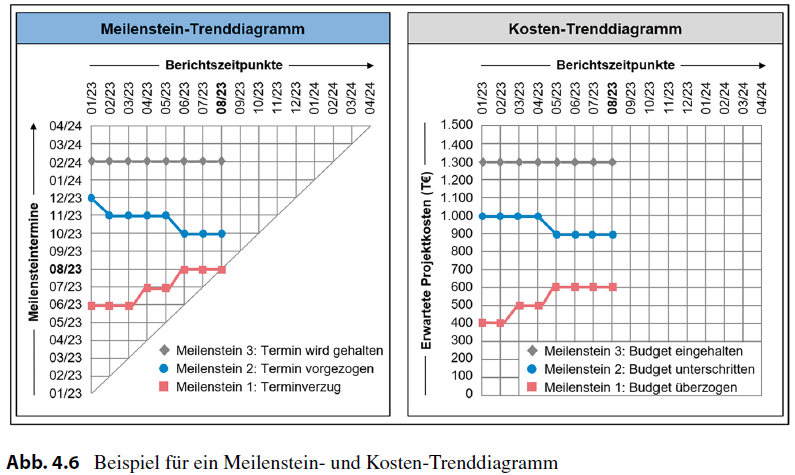
\includegraphics[width=1.1\textwidth]{BILDER-PTB4/kosten_termin.png}
\end{center}

% Anhang 2
\newpage
\phantomsection
\addcontentsline{toc}{subsection}{Anhang 2: Risikoinventars und Risk Map}
\label{sec:Anhang2}
\begin{center}
    {\Large\bfseries Anhang 2: Risikoinventars und Risk Map}\\[0.2cm]
    {\normalsize Quelle: Nonach, Kai; Zirkler, Bernd und Hofmann, Projektcontrolling: Leitfaden für die betriebliche Praxis, S. 90}\\[1.0cm]
    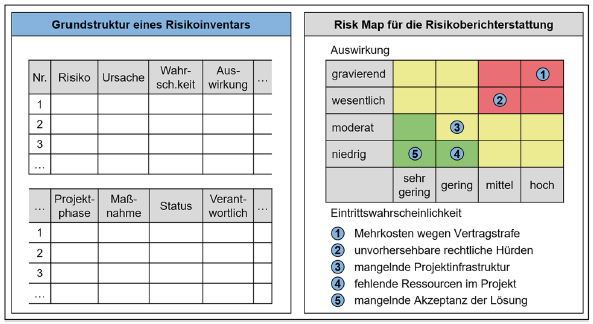
\includegraphics[width=1.1\textwidth]{BILDER-PTB4/risiko.png}
\end{center}

% Anhang 3
\newpage
\phantomsection
\addcontentsline{toc}{subsection}{Anhang 3: Burndown- und Burnup-Chart}
\label{sec:Anhang3}
\begin{center}
    {\Large\bfseries Anhang 3: Burndown- und Burnup-Chart}\\[0.2cm]
    {\normalsize Quelle: Mayrhofer, Walter und Schneikart, Gerald: Hybrides Projektmanagement: Die praktische Anwendung deterministischen und agiler Projektmanagement, S. 116}\\[1.0cm]
    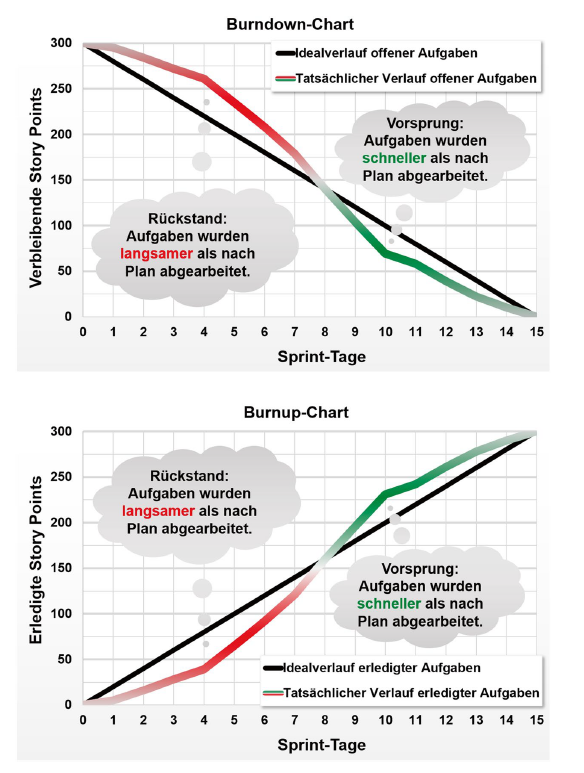
\includegraphics[width=1.0\textwidth]{BILDER-PTB4/Burndown_Chart.png}
\end{center}

% Anhang 4
\newpage
\phantomsection
\addcontentsline{toc}{subsection}{Anhang 4: Earned-Value-Analyse}
\label{sec:Anhang4}
\begin{center}
    {\large\bfseries Anhang 4: Earned-Value-Analyse}\\[0.2cm]
    {\normalsize Quelle: Mayrhofer, Walter und Schneikart, Gerald: Hybrides Projektmanagement: Die praktische Anwendung deterministischen und agiler Projektmanagement, S. 111} \\[1.0cm]
    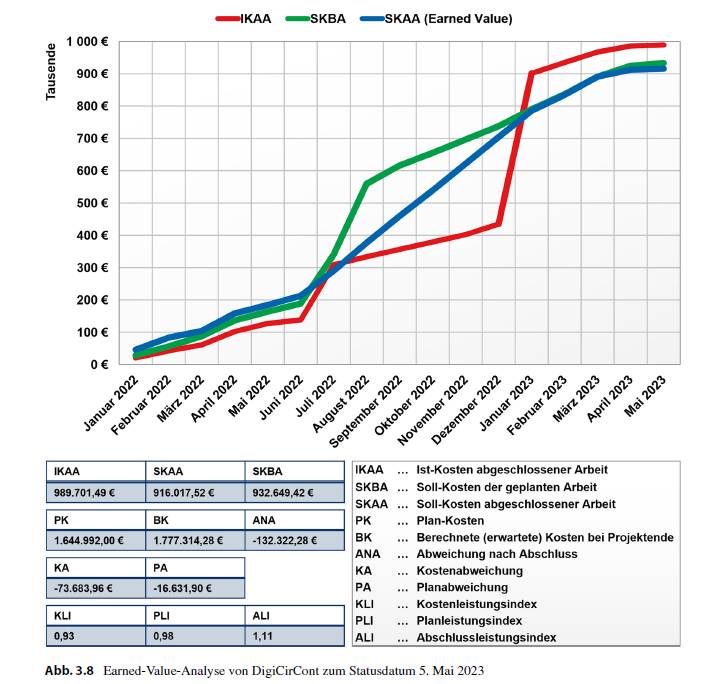
\includegraphics[width=1.1\textwidth]{BILDER-PTB4/Earned-Value-Analyse.png}
\end{center}

% Anhang 5
\newpage
\phantomsection
\addcontentsline{toc}{subsection}{Anhang 5: Interviewprotokoll (Michael Schneider)}
\label{sec:Anhang5}

{\Large\bfseries Anhang 5: Interviewprotokoll}\\[1em]
\textbf{Interviewer:} Nicole Camille Baião \\
\textbf{Befragter:} Michael Schneider (Projektleiter und Teamleiter) \\
\textbf{Datum:} 25. Juni 2026 \\
\textbf{Ort:} Berliner Wasserbetriebe, Neue J\"udenstra{\ss}e 1, 10179 Berlin

\bigskip
\noindent{\large\bfseries Anforderungen und Ziele des Projekts}

\bigskip
\noindent{\large\bfseries 1. Projektziele}

\textbf{Frage 1: Warum wollen wir SuccessFactors Learning einf\"uhren?}

Michael: Hauptgrund f\"ur das Projekt ist, dass die bisherige L\"osung IMC Learning Suite vom Hersteller IMC abgek\"undigt wurde und nicht weiterentwickelt wird. Eine neue Software wird daher zwingend ben\"otigt. Angestrebt wird eine langfristige L\"osung in Form eines Cloud-Produkts, das vom Hersteller laufend aktualisiert und an den technischen Fortschritt angepasst wird. Ziel ist die vollst\"andige \"Ubertragung der gesamten Lerneinheit in die neue Software. Aus strategischer Sicht verfolgt die IT den Ansatz, die Anzahl der eingesetzten Anwendungen zu reduzieren; da SuccessFactors bereits f\"ur Performance \& Goals sowie f\"ur Recruiting genutzt wird, soll Learning als n\"achstes Modul in dieser Standardanwendung eingef\"uhrt werden. 

Es bestehen Compliance-Anforderungen sowohl an die Softwaregestaltung allgemein als auch aus dem Learning-Bereich heraus, etwa gesetzliche Schulungspflichten aus Verordnungen und Vorschriften der Arbeitssicherheit bzw. Berufsgenossenschaft -- Beispiel: elektrisch unterwiesene Personen ben\"otigen einen j\"ahrlichen Nachweis der Unterweisung, ein Schwei{\ss}erschein f\"ur Druckrohre muss alle zwei Jahre erneuert werden. Die Auditanforderungen ergeben sich unmittelbar aus diesen Schulungspflichten: Es muss nachgewiesen werden k\"onnen, dass Mitarbeitende regelm\"a{\ss}ig geschult wurden, wof\"ur ein Auszug aus dem Learning-System als Beleg dient. Als Vorteile der neuen Software werden eine bessere Oberfl\"ache, eine einfachere Verwaltung der Seminare, ein besseres Zusammenspiel zwischen SAP HCM und SuccessFactors \"uber den Schnittstellenstandard sowie ein geringerer interner Pflegeaufwand durch die Cloud-Version erwartet.

\medskip
\textbf{Frage 2: Was sind die Erfolgskriterien des Projekts?}

Michael: Das Projekt gilt als erfolgreich, wenn die Anforderungen erf\"ullt werden -- sowohl technisch funktionsf\"ahig als auch inhaltlich passend -- und dabei kein Risiko entsteht. Ma{\ss}geblich ist das ,,magische Dreieck`` aus Zeit, Budget und Qualit\"at: Erfolg bedeutet, alle Anforderungen innerhalb der geplanten Zeit und des vorgesehenen Budgets zu erf\"ullen. Revision und Wirtschaftspr\"uferpr\"ufung sind vorhanden; s\"amtliche Projektinhalte m\"ussen in der Projektakte dokumentiert und zum Nachweis der ordnungsgem\"a{\ss}en Durchf\"uhrung archiviert werden. An das Management wird monatlich ein Statusbericht abgegeben, der den aktuellen Stand, die n\"achsten Schritte, den Zeitplan (Termintreue), den Budgetplan (Budgettreue), bestehende Risiken sowie aktuellen Entscheidungsbedarf enth\"alt.

\bigskip
\noindent{\large\bfseries 2. Projektumfang (Scope)}

\textbf{Frage 3: Welche Mitarbeiter sollen Learning nutzen?}

Michael: S\"amtliche Mitarbeitende der Berliner Wasserbetriebe arbeiten mit dem System; es gibt niemanden, der es nicht nutzt. Auch externe Dienstleister sind eingebunden, etwa externe Tutoren, die das System jedoch in der Rolle des Trainers und nicht als Lernende verwenden. Praktikantinnen und Praktikanten nehmen ebenfalls an den Unterweisungen teil.

\medskip
\textbf{Frage 4: Welche Standorte sind betroffen?}

Michael: Betroffen sind ausschlie{\ss}lich Standorte in Deutschland, da die Berliner Wasserbetriebe \"uber keine Standorte im Ausland verf\"ugen; erfasst werden dabei jedoch alle BWB-Standorte. Ob auch Tochtergesellschaften sowie Mitarbeitende von Partnerunternehmen -- etwa die Betreiber der Service-Hotline bzw. des Kundenservice -- einzubeziehen sind, muss im Projekt noch gekl\"art werden.

\medskip
\textbf{Frage 5: Welche Schulungsarten sollen unterst\"utzt werden?}

Michael: Unterst\"utzt werden sollen E-Learning, Pr\"asenzschulungen (buchbar \"uber das System), virtuelle Trainings, Webinare sowie Zertifizierungen mit entsprechenden Zertifikatsbescheinigungen. Onboarding-Schulungen sind perspektivisch, jedoch nicht sofort geplant. Pflichtschulungen sollen ebenso abgebildet werden wie externe Seminare, die \"uber das System gebucht und verwaltet werden k\"onnen sollen.

\bigskip
\noindent{\large\bfseries 3. Aktuelle Situation (Ist-Analyse)}

\textbf{Frage 6: Wie l\"auft Lernen heute?}

Michael: Aktuell im Einsatz ist die IMC Learning Suite, intern ,,Aqualern`` genannt. Verwaltung und Organisation der Schulungen erfolgen durch die Abteilung Personalf\"uhrung und -entwicklung (PTE). Teilnahmen werden im bisherigen Learning-Management-System dokumentiert; die daraus erstellten Nachweise werden von dort in die jeweilige Personalakte der Mitarbeitenden \"ubertragen. Das zentrale aktuelle Problem besteht darin, dass die Software end of life ist, nicht mehr weiterentwickelt wird und ab dem kommenden Jahr vom Hersteller nicht mehr unterst\"utzt wird.

\medskip
\textbf{Frage 7: Wie sind die Lerninhalte aufgestellt?}

Michael: E-Learning-Inhalte liegen bereits vor, \"uberwiegend im SCORM-Format, erg\"anzt um unterst\"utzende Materialien wie PDFs und PowerPoint-Pr\"asentationen. Die Inhalte werden teils bei externen Content-Anbietern eingekauft und teils intern von den jeweiligen Fachabteilungen erstellt, beispielsweise die Arbeitssicherheitsschulung durch die Abteilung ASI.

\bigskip
\noindent{\large\bfseries 4. Compliance \& Pflichtschulungen}

\textbf{Frage 8: Welche Pflichtschulungen gibt es?}

Michael: Zu den Pflichtschulungen z\"ahlen unter anderem Datenschutz und Arbeitssicherheit; die entsprechende Datenschutz-Pflichtschulung ist bereits im bisherigen System vorhanden. Grundlage sind gesetzliche Schulungspflichten, die teils unmittelbar aus dem Gesetz, teils aus Verordnungen und Vorschriften stammen -- etwa im Bereich Arbeitssicherheit bzw. von der Berufsgenossenschaft. Beispiele sind die j\"ahrliche Unterweisung elektrisch unterwiesener Personen sowie der alle zwei Jahre zu erneuernde Schwei{\ss}erschein f\"ur Druckrohre.

\medskip
\textbf{Frage 9: Welche Anforderungen bestehen an Wiederholung, Nachweis und Audits?}

Michael: Wie oft eine Schulung wiederholt werden muss, h\"angt von der jeweiligen Schulung ab: Unterweisungen erfolgen j\"ahrlich, Pflichtschulungen wie der Schwei{\ss}erschein alle zwei Jahre. F\"ur Pflichtschulungen werden grunds\"atzlich Zertifikate als Teilnahmebest\"atigung erstellt. Erinnerungen erfolgen ebenfalls schulungsabh\"angig; im heutigen Ablauf erh\"alt der Mitarbeiter bei einer ablaufenden Schulung zun\"achst einen Hinweis mit Frist, kurz danach eine weitere Erinnerung, und wird die Schulung weiterhin nicht durchgef\"uhrt, erhalten sowohl der Mitarbeiter als auch die F\"uhrungskraft einen Hinweis. Ob, wann und \"uber welche Eskalationswege erinnert wird, wird individuell je Schulung gepflegt und l\"asst sich nicht allgemein festlegen. Die Nachweise m\"ussen revisionssicher archiviert werden; dies erfolgt aktuell in der elektronischen Personalakte. Zu den relevanten Audits geh\"ort unter anderem der Audit ,,Familie und Beruf``, bei dem die Verteilung von Weiterbildungen nach Geschlecht abgefragt wird, au{\ss}erdem berichtspflichtige Meldungen nach Berlin sowie interne Kontrollen etwa zur Budgetaussch\"opfung.

\bigskip
\noindent{\large\bfseries 5. Zielgruppen \& Rollen}

\textbf{Frage 10: Wer nutzt das System?}

Michael: Das System wird von Mitarbeitenden, F\"uhrungskr\"aften, Trainern (einschlie{\ss}lich externer Tutoren), der Personalentwicklung, den Learning-Administratoren sowie einer IT-Administratorin genutzt.

\medskip
\textbf{Frage 11: Welche Aufgaben haben die Rollen?}

Michael: Mitarbeitende buchen Schulungen selbst, die Zuweisung erfolgt durch die Personalentwicklung (PME). Die Genehmigung h\"angt davon ab, ob eine Schulung kostenpflichtig ist: grunds\"atzlich genehmigen die Personalabteilung und die Weiterbildungsverantwortlichen, in der Regel zus\"atzlich die F\"uhrungskraft; bei besonders teuren Schulungen sind weitere Genehmigende einzubinden. Lernkataloge werden von der Personalabteilung (PME) erstellt, die Inhalte pflegen die jeweils zust\"andigen Referenten bzw. die Learning-Administratoren, und Berichte erstellt die Personalabteilung.

\bigskip
\noindent{\large\bfseries 6. Organisationsstruktur}

\textbf{Frage 12: Wie erfolgt die Lernzuweisung?}

Michael: Die Zuweisung von Lerninhalten erfolgt sowohl nach Abteilung als auch nach Funktion, wobei die konkrete Regelung jeweils unterschiedlich ausf\"allt.

\bigskip
\noindent{\large\bfseries 7. Integrationen}

\textbf{Frage 13: Welche SuccessFactors-Module sind vorhanden?}

Michael: Employee Central ist vorhanden, dient jedoch nur als Rahmen f\"ur die Stammdatenpflege. Recruiting sowie Performance \& Goals sind ebenfalls vorhanden. Onboarding und Compensation sind bislang nicht im Einsatz. Neu hinzukommen soll das Modul Learning.

\medskip
\textbf{Frage 14: Welche weiteren Systeme sind relevant?}

Michael: Active Directory und Microsoft Entra ID spielen an dieser Stelle keine zentrale Rolle; die Berechtigungszuweisung erfolgt \"uber das Antragssystem SMAX in Verbindung mit eDirectory, einem mit Active Directory vergleichbaren Verzeichnisdienst. SAP HCM ist die Komponente der Personalabrechnung; SAP S/4HANA sowie das \"ubrige ERP-System spielen keine Rolle, da das Personalsystem separat betrieben wird. F\"ur den Datenaustausch zwischen den SAP-Systemen dient SAP PI/PO (Process Integration / Process Orchestration) als Schnittstellensystem.

\medskip
\textbf{Frage 15: Woher kommen die Mitarbeiterdaten?}

Michael: Mitarbeiterdaten stammen urspr\"unglich aus dem SAP HCM, das dabei als f\"uhrendes System fungiert, und werden von dort an SuccessFactors \"ubergeben. Synchronisiert werden zum einen bereits vorhandene Mitarbeiterstammdaten wie Name, E-Mail-Adresse und Abteilung, zum anderen neu die Lerninhalte, etwa die Zuordnung von Pflichtschulungen. Zur\"ucksynchronisiert werden m\"ussen die Dokumente bzw. Nachweise zu absolvierten Schulungen.

\bigskip
\noindent{\large\bfseries 8. Berechtigungen \& Datenschutz}

\textbf{Frage 16: Wie ist der Datenschutz geregelt?}

Michael: Gespeichert werden personenbezogene Stammdaten wie Personalnummer und Adresse. Wer Lernhistorien und Berichte einsehen darf, muss im Projekt noch abschlie{\ss}end gekl\"art werden; grunds\"atzlich gelten jedoch Datensparsamkeit und das Need-to-know-Prinzip, wonach jeweils nur die tats\"achlich ben\"otigten Daten eingesehen werden d\"urfen und der Umfang je Bericht unterschiedlich ausf\"allt, etwa begrenzt auf F\"uhrungsgrenzen oder einen eingeschr\"ankten Personenkreis. Zust\"andig f\"ur die Mitbestimmung ist der Personalrat, nicht der Betriebsrat; dieser stellt Anforderungen insbesondere in Richtung Datenschutz und ergonomischer Softwaregestaltung und muss der Einf\"uhrung zustimmen.

\bigskip
\noindent{\large\bfseries 9. Projektorganisation}

\textbf{Frage 17: Wer ist Auftraggeber und wer trifft Entscheidungen?}

Michael: Auftraggeber des Projekts ist die Personalabteilung bzw. das Personalmanagement. Entscheidungen trifft die Projektleitung in Abstimmung mit dem Personalmanagement und der Leitung IT; das Budget genehmigen die Leitung IT und das Personalmanagement gemeinsam.

\medskip
\textbf{Frage 18: Wie ist das Projektteam zusammengesetzt?}

Michael: Das Projektteam besteht aus Projektleitung, HR-Vertretung, Learning-Spezialisten und IT-Vertretung. Der Datenschutz wird bei Bedarf einbezogen, ist jedoch kein st\"andiges Mitglied des Projektteams. Der Personalrat ist als Beteiligter einzubinden, geh\"ort aber ebenfalls nicht zum Projektteam. Compliance ist nicht beteiligt, ebenso wenig die einzelnen Fachbereiche, die sp\"ater lediglich als Teilnehmende der Schulungen auftreten.

\medskip
\textbf{Frage 19: Wird externe Unterst\"utzung hinzugezogen?}

Michael: Als Implementierungspartner fungiert die Firma Sopra Steria, ein Rahmenvertragspartner im SuccessFactors-Umfeld. Die Konfiguration \"ubernehmen die BWP-IT-Kolleginnen und -Kollegen gemeinsam mit dem Implementierungspartner Sopra Steria.

% Anhang 6
\newpage
\phantomsection
\addcontentsline{toc}{subsection}{Anhang 6: Interviewprotokoll (Jonathan Scheidel)}
\label{sec:Anhang6}

{\Large\bfseries Anhang 6: Interviewprotokoll}\\[1em]
\textbf{Interviewer:} Nicole Camille Bai\~ao \\
\textbf{Befragter:} Jonathan Scheidel (Personalentwickler, Auftraggeber) \\
\textbf{Datum:} 30. Juni 2026 \\
\textbf{Ort:} Berliner Wasserbetriebe, Neue J\"udenstra{\ss}e 1, 10179 Berlin

\bigskip
\noindent{\large\bfseries Erg\"anzende Anforderungen aus dem Personalmanagement (PM)}

\bigskip
\noindent{\large\bfseries 1. Berechtigungen \& Datenschutz}

\textbf{Frage 1: Wer darf Lernhistorien sehen?}

Jonathan: Aus Sicht der Personalentwicklung sollte die Lernhistorie f\"ur die Besch\"aftigten selbst sowie f\"ur die F\"uhrungskraft einsehbar sein, ebenso f\"ur die Weiterbildungsbeauftragten, die als dezentrale Rolle in den Bereichen f\"ur die Weiterbildung zust\"andig sind und als erste bzw. zweite Ansprechperson nach der F\"uhrungskraft fungieren. Aktuell ist dies aus Datenschutzgr\"unden bereits eingeschr\"ankt worden: F\"uhrungskr\"afte k\"onnen die Lernhistorie ihrer Besch\"aftigten derzeit nicht mehr einsehen, einsichtsberechtigt sind nur noch die Weiterbildungsbeauftragten zentral, an die sich F\"uhrungskr\"afte bei Bedarf wenden m\"ussen. F\"ur das neue System besteht der Wunsch, das Thema erneut aufzugreifen und den F\"uhrungskr\"aften wieder Zugriff zu erm\"oglichen; dieser Zielzustand soll als Anforderung aufgenommen werden, die datenschutzrechtliche Umsetzbarkeit ist separat zu pr\"ufen.

\medskip
\textbf{Frage 2: Wer darf Berichte sehen?}

Jonathan: Berichte werden als Gesamtauswertungen f\"urs Controlling bzw. zum Jahresende verstanden. Personalberichte sollten grunds\"atzlich nur von der Personalentwicklung (PME) eingesehen und reportet werden k\"onnen. Weiterbildungsbeauftragte sollten f\"ur ihren eigenen Verantwortungsbereich Einsicht erhalten, etwa in die Anzahl offener bzw. abgeschlossener Seminare. F\"uhrungskr\"afte ben\"otigen dies nicht zwingend, k\"onnten jedoch f\"ur den eigenen Bereich profitieren, insbesondere f\"ur das Budget-Reporting. Zentral bzw. kurs\"ubergreifend liegt die Zust\"andigkeit bei der Personalentwicklung.

\medskip
\textbf{Frage 3: Welche Administratorrollen gibt es?}

Jonathan: Der aktuelle Stand unterscheidet sich vom k\"unftig gew\"unschten. Vorgesehen ist ein Super-Admin bzw. IT-Fachadmin mit s\"amtlichen Funktionen und Berechtigungen im System. Darunter soll ein Fachadministrator angesiedelt sein, besetzt durch die Personalentwicklung sowie ein bis zwei Personen aus der Ausbildung; dieser kann Kurse konfigurieren, Reporting durchf\"uhren, Berechtigungen verwalten und allgemeines Mailing anpassen, verf\"ugt jedoch \"uber weniger Rechte als der Super-Admin. Darunter sind die Inhalts-Administratoren bzw. Trainer angesiedelt, die selbst Inhalte erstellen k\"onnen. Dar\"uber hinaus wird es vermutlich noch Rollen f\"ur Controller und F\"uhrungskr\"afte geben.

\medskip
\textbf{Frage 4: Wer darf Inhalte erstellen?}

Jonathan: Aktuell obliegt dies den Inhalts-Administratoren; k\"unftig k\"onnten diese als ,,Trainer`` bezeichnet werden.

\medskip
\textbf{Frage 5: Wer darf Berichte erzeugen?}

Jonathan: Berichte erzeugen k\"onnen F\"uhrungskr\"afte und Weiterbildungsbeauftragte sowie zentrale bzw. dezentrale Controller in den Bereichen, die f\"ur das Budget verantwortlich sind. Zus\"atzlich sind die Personalentwicklung zentral sowie die Abteilung Ausbildung berichtsberechtigt.

\medskip
\textbf{Frage 6: Wer darf Pflichtschulungen zuweisen?}

Jonathan: Pflichtschulungen sind in den jeweiligen Verantwortungsbereichen verortet; Compliance-Pflichtschulungen kommen beispielsweise vom Bereich Corporate Governance (Team Compliance), der auch f\"ur deren Zuweisung verantwortlich ist. Technisch h\"atten auch die Inhalts-Administratoren bzw. die Trainerrolle die M\"oglichkeit, Pflichtschulungen zuzuweisen; dies birgt jedoch das Risiko einer versehentlichen unternehmensweiten Zuweisung. Aktuell wird das eher kommunikativ gel\"ost, da im Lernmanagementsystem eine Schulung heute nicht technisch als ,,verpflichtend f\"ur alle`` hinterlegt ist. K\"unftig wird eine st\"arkere zentrale Kontrolle bzw. Freigabe durch die Personalentwicklung gew\"unscht, damit nicht jede Abteilung eigenst\"andig unternehmensweite Pflichtschulungen anlegen kann. Betroffen sind aktuell nur wenige Abteilungen, insbesondere Corporate Governance und Arbeitssicherheit, perspektivisch eventuell auch Strategie/Unternehmensentwicklung und Unternehmenssicherheit.

\bigskip
\noindent{\large\bfseries 2. Reporting \textendash{} ben\"otigte Berichte}

\textbf{Frage 7: Welche Berichte zu offenen Pflichtschulungen werden ben\"otigt?}

Jonathan: Berichte zu offenen Pflichtschulungen sind vor allem f\"ur die verantwortlichen Fachbereiche relevant, etwa Corporate Governance beim Compliance-Kurs oder Arbeitssicherheit bei der entsprechenden Schulung. Ben\"otigt wird eine \"Ubersicht, welche Personen einen Kurs noch nicht abgeschlossen haben und bis wann dieser abgeschlossen sein muss, da feste Fristen bestehen, etwa vier oder acht Wochen nach Kurs\"offnung. F\"ur die Abteilung Personalgrundsatz sind diese Daten relevant, um m\"ogliche arbeitsrechtliche Konsequenzen bei Nichtabsolvieren zu bewerten, was aktuell teils noch h\"andisch erfolgt. Grundlegend ben\"otigt wird eine Liste der Personen, die den Kurs bereits absolviert haben, sowie eine Liste der noch offenen Personen.

\medskip
\textbf{Frage 8: Welche Berichte zu abgelaufenen Zertifizierungen werden ben\"otigt?}

Jonathan: Relevant ist dies vor allem auf Ebene j\"ahrlich wiederkehrender Turnusschulungen. Gew\"unscht wird ein Kursfortschritts- bzw. Abschlussbericht f\"ur Pflichtschulungen sowie ein Bericht zu offenen bzw. nicht abgeschlossenen Pflichtschulungen. Derartige Berichte gibt es vermutlich bereits standardm\"a{\ss}ig in anderen Systemen.

\medskip
\textbf{Frage 9: Wie soll der Compliance-Status abgebildet werden?}

Jonathan: Der Compliance-Status wird als Anteil der Besch\"aftigten verstanden, die eine bestimmte Pflichtschulung, etwa den Compliance-Kurs, absolviert haben (Beispiel: 90 Prozent Compliance-Status). Diese Auswertung sollte pro Kurs m\"oglich sein, beispielsweise f\"ur den Bereich Corporate Governance/Compliance.

\medskip
\textbf{Frage 10: Welche Dashboards werden ben\"otigt?}

Jonathan: Welche Dashboards ben\"otigt werden, h\"angt von der jeweiligen Rolle ab. F\"ur die Personalentwicklung wird ein zentrales Dashboard mit sinnvollen Kennzahlen gew\"unscht. Auch F\"uhrungskr\"afte, Weiterbildungsbeauftragte und Controller ben\"otigen f\"ur ihren jeweiligen Bereich eine Auswertung auf einen Blick, etwa zu Teilnehmerzahlen und entstandenen Kosten.

\bigskip
\noindent{\large\bfseries 3. Zielgruppen, Mitarbeitergruppen \& Sonderf\"alle}

\textbf{Frage 11: Gibt es unterschiedliche Mitarbeitergruppen mit unterschiedlichem Schulungsbedarf?}

Jonathan: Es gibt unterschiedliche Mitarbeitergruppen mit individuellem Schulungsbedarf, beispielsweise ben\"otigen technisch-gewerbliche Besch\"aftigte andere Sicherheitsunterweisungen und Atemschutzschulungen als B\"urobesch\"aftigte. Dies ist nur ein Beispiel von mehreren Gruppen mit jeweils eigenen Anforderungen.

\medskip
\textbf{Frage 12: Wie werden befristet Besch\"aftigte, Auszubildende und duale Studierende ber\"ucksichtigt?}

Jonathan: Auszubildende und duale Studierende werden von der Abteilung Ausbildung betreut, die Teil des Personalmanagements ist. Die Abteilung Ausbildung verf\"ugt \"uber eigene Systemzug\"ange mit Admin-Rolle und kann das System konfigurieren; sie bietet eigene, zielgruppenspezifische Kursangebote f\"ur Auszubildende und duale Studierende an, analog zu den Angeboten f\"ur regul\"are Besch\"aftigte, und ist f\"ur diese Zielgruppe verantwortlich. Befristet Besch\"aftigte werden dagegen wie regul\"are Besch\"aftigte behandelt, ohne gesonderte Unterscheidung.

\medskip
\textbf{Frage 13: Wie sollen Mitarbeitende ohne festen PC-Arbeitsplatz Schulungen absolvieren?}

Jonathan: Bisher fahren zust\"andige Verantwortliche, etwa aus dem Compliance-Bereich, ins Werk und stellen vor Ort Zeit sowie Tablets oder PCs zur Verf\"ugung. Grunds\"atzlich sehen die Dienstvereinbarungen, unter anderem zum mobilen Arbeiten, vor, dass alle Besch\"aftigten Zugang zu einem PC-Arbeitsplatz haben, der nicht fest zugeordnet sein muss. In Bereichen ohne Einzelger\"ate gibt es Poolger\"ate im Schl\"ussel von etwa einem Ger\"at pro f\"unf bis zehn Besch\"aftigte, die untereinander aufgeteilt werden.

\medskip
\textbf{Frage 14: Wie wird mit ablaufenden Pflichtschulungen bei Elternzeit oder Langzeiterkrankung umgegangen?}

Jonathan: Perspektivisch soll die Bearbeitung nach R\"uckkehr erfolgen; Teilnehmende werden informiert, dass die zeitnahe Absolvierung erforderlich ist. In der Praxis erfolgt der entsprechende Hinweis meist \"uber die F\"uhrungskraft direkt bei R\"uckkehr. Das aktuelle System bietet dabei eingeschr\"ankte M\"oglichkeiten im Vergleich zu anderen Systemen. Gew\"unscht wird f\"ur das neue System ein automatischer, kursbezogener Turnus, etwa ein Jahr G\"ultigkeit ab Teilnahmezertifikat, mit automatischer Erinnerung durch das System bei erneuter F\"alligkeit.

\bigskip
\noindent{\large\bfseries 4. Schulungsbedarf \& Schulungskonzept}

\textbf{Frage 15: Wer ermittelt den j\"ahrlichen Schulungsbedarf je Abteilung bzw. Funktion?}

Jonathan: Der Ermittlungsweg h\"angt von der Art der Inhalte ab. Pflichtthemen kommen aus den jeweiligen Bereichen selbst, wof\"ur die Weiterbildungsbeauftragten verantwortlich sind. Der \"ubrige Bedarf wird in der Regel im Zielvereinbarungsgespr\"ach festgelegt, in dem neben Kompetenzen auch Schulungen vereinbart werden. Unterj\"ahrig stellt die Personalentwicklung zus\"atzliche Inhalte im Aqualearn als Add-on bereit.

\medskip
\textbf{Frage 16: Gibt es bereits ein Kompetenz- oder Qualifikationsmodell?}

Jonathan: Es existiert bereits das CODE-Kompetenzmodell des Anbieters KODE (Kompetenz, Diagnostik und Entwicklung). Es umfasst ein Gesamtkompetenzmodell mit 64 Teilkompetenzen, heruntergebrochen auf aktuell etwa 16 bis 18 Kompetenzen f\"ur Besch\"aftigte bzw. F\"uhrungskr\"afte. Diese Kompetenzen lassen sich als Tags bzw. Labels an Kursen hinterlegen, sodass beispielsweise ein Kurs zum Thema Storytelling auf die Kommunikationskompetenz einzahlt. Qualifikationen im engeren Sinn, etwa Qualifikationspfade, werden bislang eher nicht eingesetzt, lie{\ss}en sich aber im Sinne der Personalentwicklungspl\"ane (PEP) verstehen, f\"ur die bereits ein vorgefertigtes Qualifikationsmodell existiert.

\medskip
\textbf{Frage 17: Wie sollen individuelle Entwicklungspl\"ane mit dem Lernkatalog verbunden werden?}

Jonathan: Sinnvoll erscheint es, Kompetenzen wie bisher im Zielvereinbarungs- bzw. Mitarbeitergespr\"ach festzulegen. Die Verkn\"upfung wird als grunds\"atzlich einfach umsetzbar eingesch\"atzt: In SuccessFactors hinterlegte, im kommenden Jahr zu entwickelnde Kompetenzen sollen im Aqualearn passende Kursvorschl\"age ausl\"osen. Gew\"unscht wird zudem, dass Besch\"aftigte im Aqualearn eigenst\"andig nach Tags bzw. Kompetenz-Labels filtern k\"onnen, im Idealfall mit automatischem Vorschlag passender Kurse.

\medskip
\textbf{Frage 18: Soll es eine Verkn\"upfung zwischen Performance \& Goals und den empfohlenen Lerninhalten geben?}

Jonathan: Eine Verkn\"upfung zwischen Performance \& Goals und den empfohlenen Lerninhalten wird grunds\"atzlich gew\"unscht, da sich viele Inhalte ohnehin am Kompetenzmodell orientieren und das Zielvereinbarungsgespr\"ach bereits zielorientiert abl\"auft.

\bigskip
\noindent{\large\bfseries 5. Rollen, Verantwortlichkeiten \& Genehmigungsprozesse}

\textbf{Frage 19: Wer vertritt die Personalentwicklung bei Abwesenheit in der Zuweisung von Pflichtschulungen?}

Jonathan: Aktuell ist die Zuweisung von Pflichtschulungen nicht direkt Aufgabe der Personalentwicklung. Perspektivisch ist eine ,,Zwischenrolle`` denkbar, die diese Aufgabe \"ubernehmen k\"onnte, ohne dass dies bereits konkret definiert ist. Eine klassische Vertretungsregelung wird nicht als zwingend notwendig angesehen, da grunds\"atzlich mehrere Personen, etwa Admins, diese Aufgabe \"ubernehmen k\"onnten. Pflichtschulungen sollen grunds\"atzlich eher aus den Fachbereichen kommen, etwa Corporate Governance oder Arbeitssicherheit; die Personalentwicklung agiert dabei eher als Freigabeinstanz.

\medskip
\textbf{Frage 20: Welche Eskalationsstufen gibt es bei nicht genehmigten oder nicht bearbeiteten Schulungen?}

Jonathan: Konkrete Eskalationsstufen sind aktuell nicht abschlie{\ss}end bekannt. Bekannt ist, dass bei nicht absolvierten Pflichtschulungen gemeinsam mit der Abteilung Corporate Governance bzw. Grundsatzabteilung gepr\"uft wurde, dass grunds\"atzlich arbeitsrechtliche Konsequenzen m\"oglich sind; die konkrete Ausgestaltung ist nicht bekannt. Die Arbeitnehmervertretung unterst\"utzt in diesem Zusammenhang.

\bigskip
\noindent{\large\bfseries 6. Pflichtschulungen, Fristen \& Eskalation}

\textbf{Frage 21: Wer legt fest, welche Mitarbeitergruppe welche Pflichtschulung ben\"otigt?}

Jonathan: Meist ist die Zuordnung eindeutig, etwa erhalten Besch\"aftigte, die mit gesundheitssch\"adlichen Gasen arbeiten, eine Atemschutzschulung. Die Festlegung erfolgt durch die Weiterbildungsbeauftragten bzw. F\"uhrungskr\"afte der jeweiligen Bereiche. Ansonsten wird im Wesentlichen nur zwischen zwei groben Gruppen unterschieden, F\"uhrungskr\"aften und Besch\"aftigten, die \"uber das System einfach adressierbar sind; eine weitergehende Differenzierung nach zus\"atzlichen Mitarbeitergruppen findet nicht statt.

\medskip
\textbf{Frage 22: Wie wird mit neuen, unterj\"ahrig eingef\"uhrten Pflichtschulungen umgegangen?}

Jonathan: Neue Pflichtschulungen k\"onnen unterj\"ahrig eingef\"uhrt werden und sind nicht immer langfristig im Voraus geplant. Der Zeitraum zur Absolvierung wird dann entsprechend angepasst, beispielsweise auf den Zeitraum Juni bis September statt zum Jahresende. Dies wird nicht als Problem angesehen.

\medskip
\textbf{Frage 23: Wer ist verantwortlich, wenn eine Pflichtschulung trotz Eskalation nicht abgeschlossen wird?}

Jonathan: Verantwortlich ist der Fachbereich, der die Pflichtschulung eingerichtet hat; dieser geht auf die betroffene F\"uhrungskraft zu. Die F\"uhrungskraft ist daf\"ur verantwortlich, dass die Besch\"aftigten die Schulung absolvieren, und wird als erste Stelle adressiert.

\medskip
\textbf{Frage 24: Wie werden R\"uckfragen oder Ausnahmeantr\"age zu Pflichtschulungen bearbeitet?}

Jonathan: Jeder Kurs verf\"ugt \"uber eine verantwortliche Administration bzw. Ansprechperson, die im Kurs mit Bild, E-Mail-Adresse und Telefonnummer hinterlegt ist; diese Person wird bei R\"uckfragen oder Ausnahmeantr\"agen kontaktiert. Perspektivisch w\"aren mehrere parallele Kommunikationswege, etwa E-Mail und Telefon, vorstellbar.

\bigskip
\noindent{\large\bfseries 7. Lernkatalog \& Content-Management}

\textbf{Frage 25: Wer entscheidet \"uber die Aufnahme neuer externer Lerninhalte in den Katalog?}

Jonathan: Die Personalentwicklung entscheidet \"uber die Aufnahme, in Abstimmung mit dem jeweiligen Fachbereich. Bei Interesse eines Fachbereichs an neuen Inhalten erfolgt eine gemeinsame Pr\"ufung mit dem Datenschutz, ob und wie eine Einbindung m\"oglich ist. Die Personalentwicklung \"ubernimmt anschlie{\ss}end die inhaltliche Pr\"ufung sowie die technische Umsetzung; das Content-Management liegt zentral bei der Personalentwicklung, da dort der \"Uberblick \"uber den Gesamtkatalog vorhanden ist.

\medskip
\textbf{Frage 26: Wie oft werden bestehende Lerninhalte auf Aktualit\"at gepr\"uft?}

Jonathan: Jeder Kurs verf\"ugt \"uber ein hinterlegtes Enddatum, das eher konservativ bzw. kurz gepflegt wird; Kurse mit einer G\"ultigkeit \"uber mehrere Jahre sind selten. F\"ur die Aktualit\"at ist die jeweils verantwortliche Person je Kurs zust\"andig. In der Praxis melden Besch\"aftigte, die selbst Fachpersonal sind und den Kurs absolvieren, Unstimmigkeiten direkt an die zust\"andige Administration, die daraufhin \"Anderungen vornimmt.

\medskip
\textbf{Frage 27: Gibt es einen Freigabeprozess f\"ur neue oder ge\"anderte Lerninhalte vor Ver\"offentlichung?}

Jonathan: Es gilt ein tendenzielles Vier-Augen-Prinzip: Die Fachabteilung erstellt Inhalte, die Personalentwicklung pr\"uft diese gegen, vor allem didaktisch und nicht fachlich-inhaltlich, da Fachpersonen oft nicht didaktisch geschult sind. H\"aufig erfolgt zus\"atzlich eine Pr\"ufung durch die F\"uhrungskraft des jeweiligen Bereichs. Die Arbeitnehmervertretung muss laut der neuen Dienstvereinbarung E-Learning nicht mehr zustimmen, wird jedoch \"uber neue Lerninhalte informiert. Vereinzelt erstellen Fachbereiche eigenst\"andig Inhalte, meist duplizierte Inhalte aus Vorjahren, die anschlie{\ss}end mit der F\"uhrungskraft abgestimmt werden. F\"ur die Ausbildung wird ein eigener, angepasster Prozess ben\"otigt, da dort m\"oglicherweise eine andere Beteiligung erforderlich ist.

\bigskip
\noindent{\large\bfseries 8. Zertifizierungen \& Qualifikationsmanagement}

\textbf{Frage 28: Welche Informationen muss ein Zertifikat zwingend enthalten?}

Jonathan: Es handelt sich meist nicht um Zertifikate im engeren Sinne, sondern um Teilnahmebest\"atigungen, da in den seltensten F\"allen eine Wissensabfrage oder Pr\"ufung am Ende erfolgt. Eine Teilnahmebest\"atigung enth\"alt in der Regel Ausstelldatum bzw. G\"ultigkeitsdauer sowie die ausstellende Person und ist meist ein Jahr g\"ultig. Die G\"ultigkeitsdauer ist aktuell nicht durchg\"angig hinterlegt; dies soll k\"unftig erg\"anzt werden, insbesondere bei Pflichtthemen.

\medskip
\textbf{Frage 29: Wie werden externe Zertifikate ins System eingepflegt?}

Jonathan: Dies wird sehr unterschiedlich gehandhabt: Externe Anbieter versenden Teilnahmebest\"atigungen h\"aufig separat, losgel\"ost vom System, teils per Upload in eine Bibliothek, teils per Mail aus dem Aqualearn heraus. Die meisten externen Schulungen haben gar keine Ber\"uhrung mit dem Aqualearn, da sie zentral \"uber die Personalentwicklung gepflegt werden. Bei Rahmenvertr\"agen mit externen Anbietern arbeitet der Anbieter direkt im Aqualearn und l\"adt entweder eine automatisch generierte oder eine eigene Teilnahmebest\"atigung hoch.

\medskip
\textbf{Frage 30: Wer pr\"uft die G\"ultigkeit und Echtheit externer Nachweise?}

Jonathan: Aktuell pr\"uft dies niemand konkret. \"Uber die Personalakte l\"asst sich nachvollziehen, dass eine Teilnahme stattgefunden hat, ein eigentlicher Echtheitscheck erfolgt jedoch nicht. Zust\"andig w\"are am ehesten der jeweilige Fachbereich, da eine zentrale Instanz wie die Personalentwicklung dies nicht f\"ur alle Bereiche pr\"ufen bzw. bescheinigen kann.

\bigskip
\noindent{\large\bfseries 9. Onboarding \& Verkn\"upfung mit anderen HR-Prozessen}

\textbf{Frage 31: Welche Schulungen sollen verpflichtend Teil des Onboarding-Prozesses sein?}

Jonathan: Der Onboarding-Prozess ist im Aqua.net hinterlegt und wird gelegentlich um neue Inhalte der Personalentwicklung erg\"anzt. Verpflichtend ist unter anderem eine F\"uhrungskr\"afte-Basiswissen-Schulung mit j\"ahrlichem Turnus. F\"ur Besch\"aftigte geh\"oren grundlegende Themen wie Internetnutzung dazu. Eine Standardschulung zum mobilen Arbeiten sowie der digitale F\"uhrerschein, ein Angebot f\"ur Personen mit digitalen Einstiegsschwierigkeiten, sind hingegen nur Empfehlungen und keine Pflichtkurse.

\medskip
\textbf{Frage 32: Bis zu welchem Zeitpunkt m\"ussen Onboarding-Schulungen abgeschlossen sein?}

Jonathan: Dies wird aktuell nicht eng nachverfolgt; die Verantwortung liegt bei der F\"uhrungskraft bzw. der jeweils zust\"andigen Trainingsinstanz und h\"angt vom jeweiligen Training ab, etwa wenn externe Anbieter nur alle drei bis sechs Monate Kurse durchf\"uhren. Rein online-basierte Pflichtschulungen sollen voraussichtlich innerhalb der ersten zwei Wochen absolviert werden.

\bigskip
\noindent{\large\bfseries 10. Reporting \& Kennzahlen aus PM-Sicht}

\textbf{Frage 33: In welcher Frequenz ben\"otigt PM eigene interne Auswertungen?}

Jonathan: Am liebsten w\"urden Auswertungen bei Bedarf bzw. sofort bei Systemzugriff zur Verf\"ugung stehen. Regelm\"a{\ss}ig ist mindestens eine quartalsweise Auswertung erforderlich. W\"ochentliche oder monatliche Auswertungen werden voraussichtlich nicht ben\"otigt. Gew\"unscht wird ein selbstst\"andiges, tagesaktuelles Ziehen von Reports auf Knopfdruck anstelle automatisch zugestellter Reports.

\bigskip
\noindent{\large\bfseries 11. Budget \& Ressourcenplanung}

\textbf{Frage 34: Wie wird das j\"ahrliche Weiterbildungsbudget auf die Abteilungen verteilt?}

Jonathan: Die Personalentwicklung erh\"alt das Gesamtbudget f\"ur das Jahr und muss es auf zentrale sowie dezentrale Weiterbildungsthemen aufteilen. Die Verteilung erfolgt anhand historischer Werte, etwa des Budgetverbrauchs der jeweiligen Abteilung im Vorjahr und der Aussch\"opfung angemeldeter Budgets, sowie unter Ber\"ucksichtigung der Abteilungsgr\"o{\ss}e. Technisch-gewerbliche Abteilungen erhalten tendenziell weniger Budget pro Person, da die Schulungskosten dort meist g\"unstiger sind als etwa bei IT- oder Ingenieur-Weiterbildungen. Die weitere Verteilung erfolgt \"uber die Bereiche bzw. Organisationseinheiten, die das Budget intern nochmals herunterbrechen.

\medskip
\textbf{Frage 35: Wer entscheidet, wenn das Budget f\"ur externe Seminare in einem Bereich \"uberschritten wird?}

Jonathan: Die Information \"uber eine Budget\"uberschreitung geht an die Personalentwicklung, die den betroffenen Bereich adressiert und bittet, die Notwendigkeit nochmals zu pr\"ufen. Eine Entscheidungshoheit \"uber das Budget der Bereiche selbst hat die Personalentwicklung nicht; die Freigabe zur \"Uberziehung erfolgt in der Regel durch das Management bzw. die F\"uhrungskraft des jeweiligen Bereichs.

\bigskip
\noindent{\large\bfseries 12. Kommunikation \& Change Management}

\textbf{Frage 36: Welche Informationskan\"ale nutzt PM, um Mitarbeitende \"uber Pflichtschulungen zu informieren?}

Jonathan: Aqua.net ist der Hauptkanal f\"ur kaufm\"annische Bereiche, technisch-gewerbliche Bereiche werden zus\"atzlich verst\"arkt per E-Mail informiert. Meist erfolgt die Information \"uber die F\"uhrungskraft, die regelm\"a{\ss}ig auf die Mailbox zugreift und die Information an die Besch\"aftigten weitergibt, was jedoch nicht f\"ur alle Besch\"aftigten gleicherma{\ss}en gilt. Alternativ erfolgt die Verteilung \"uber Sekretariate, an die eine Mail geschickt wird, die diese dann intern weiterverteilen, insbesondere f\"ur Besch\"aftigte ohne regelm\"a{\ss}igen Mailbox-Zugriff. Gelegentlich werden zus\"atzlich Frage-Antwort-Formate wie Teams-Meetings angeboten, deren Ank\"undigung ebenfalls \"uber Aqua.net erfolgt.

\medskip
\textbf{Frage 37: Soll es eine Pilotgruppe vor dem unternehmensweiten Rollout geben?}

Jonathan: F\"ur das neue System soll es eine Pilotgruppe vor dem unternehmensweiten Rollout geben. Vorgesehen ist der Einsatz des bestehenden Anwenderkreises an Heavy-Usern, teilweise Weiterbildungsbeauftragte, teilweise interne Trainer, die das System testen und an ihre jeweiligen Zielgruppen weitergeben sollen. Dazu z\"ahlen auch Personen aus technisch-gewerblichen Bereichen, die diese Zielgruppe gezielt einbinden k\"onnen, da sie bei bisherigen Angeboten oft zu wenig ber\"ucksichtigt wurde.

% Anhang 7
\newpage
\phantomsection
\addcontentsline{toc}{subsection}{Anhang 7: Projektphasen - Meilensteinsplan}
\label{sec:Anhang7}
\begin{center}
    {\Large\bfseries Anhang 7: Projektphasen - Meilensteinsplan}\\[0.2cm]
    {\normalsize interne Quelle von Berliner Wasserbetriebe}\\[1.0cm]
    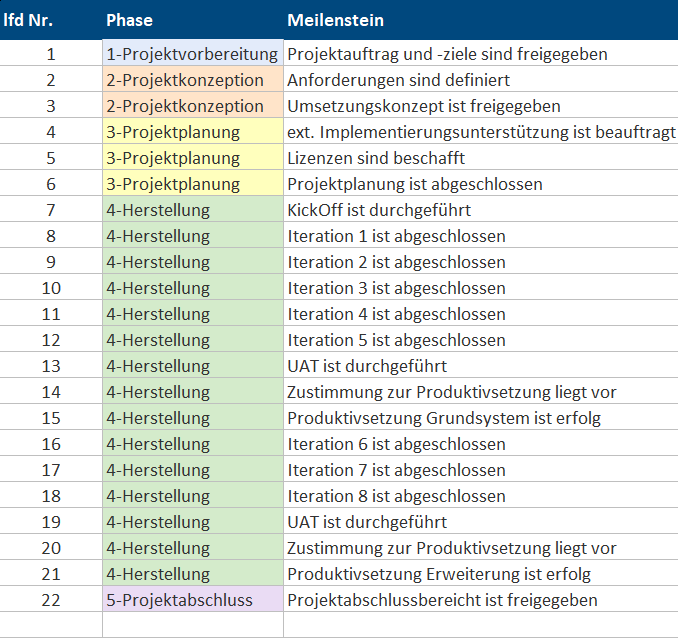
\includegraphics[width=1.1\textwidth]{BILDER-PTB4/Phasen.png}
\end{center}

% Anhang 8
\newpage
\phantomsection
\addcontentsline{toc}{subsection}{Anhang 8: Termincontrolling bei den BWB}
\label{sec:Anhang8}
\vspace*{\fill}
\begin{center}
    \begin{adjustbox}{rotate=90, center, valign=b}
        \begin{minipage}{0.95\textheight}
            \centering
            {\Large\bfseries Anhang 8: Termincontrolling bei den BWB}\\[1em]
             {\normalsize Quelle: Eigene Darstellung in Anlehnung an die Projektphasen bei den BWB}\\[0.4cm]
            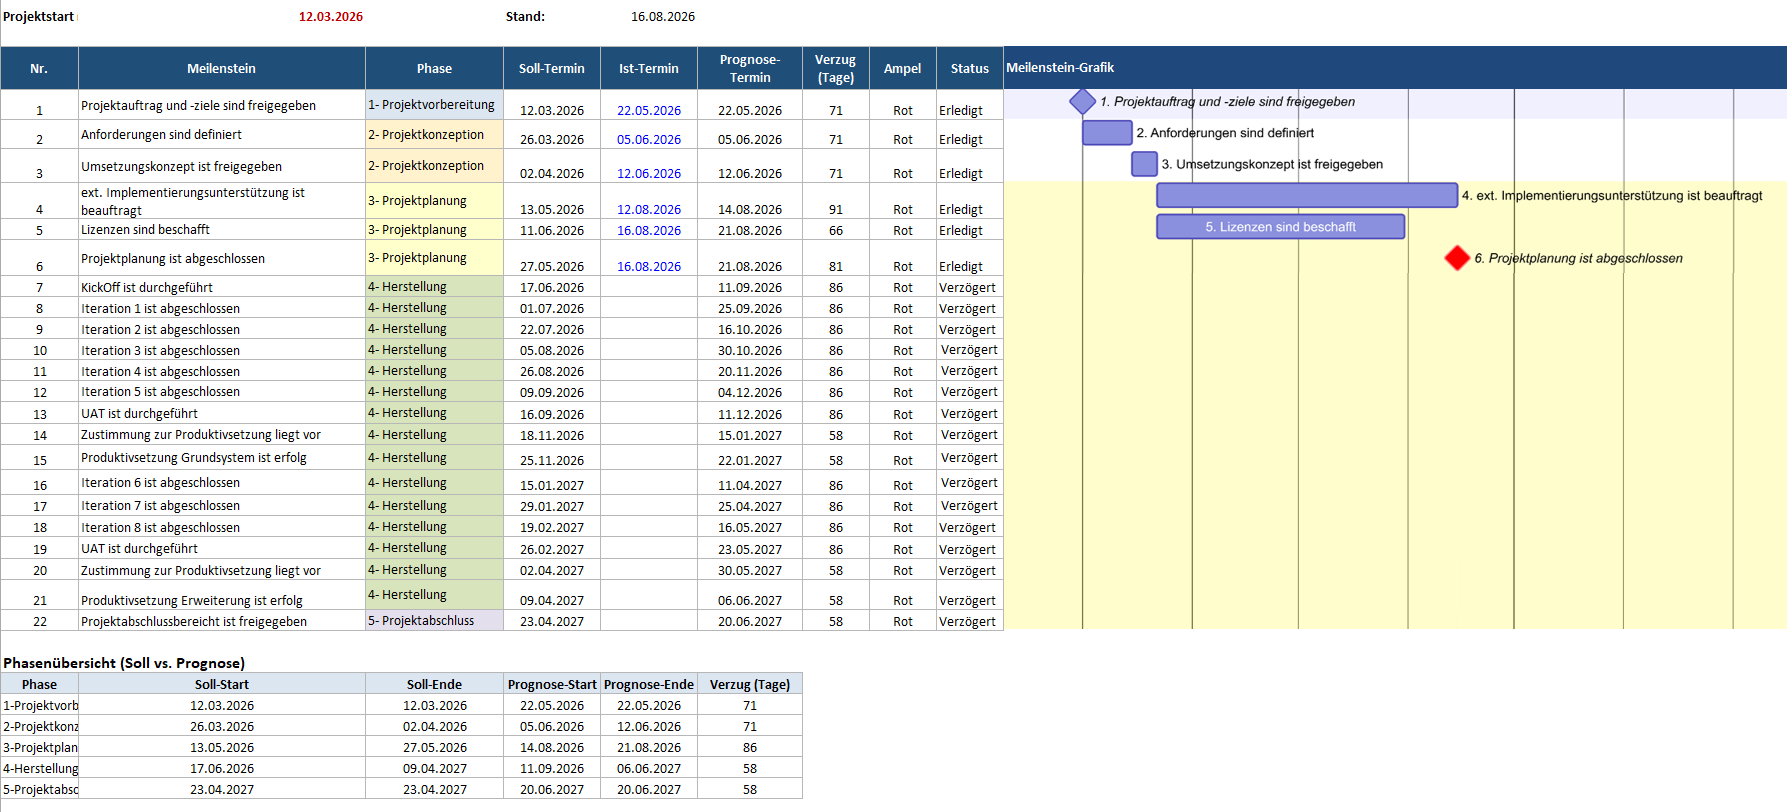
\includegraphics[width=0.9\textheight,keepaspectratio]{BILDER-PTB4/Termincontrolling_mit_Grafik.png}
        \end{minipage}
    \end{adjustbox}
\end{center} 

% Anhang 9
\newpage
\phantomsection
\addcontentsline{toc}{subsection}{Anhang 9: Projektkosten}
\label{sec:Anhang9}
\begin{center}
    {\Large\bfseries Anhang 9: Projektkosten}\\[0.2cm]
    {\normalsize interne Quelle: Projektkostensdokument (Ablösung Learning Management System) bei den BWB}\\[1.0cm]
    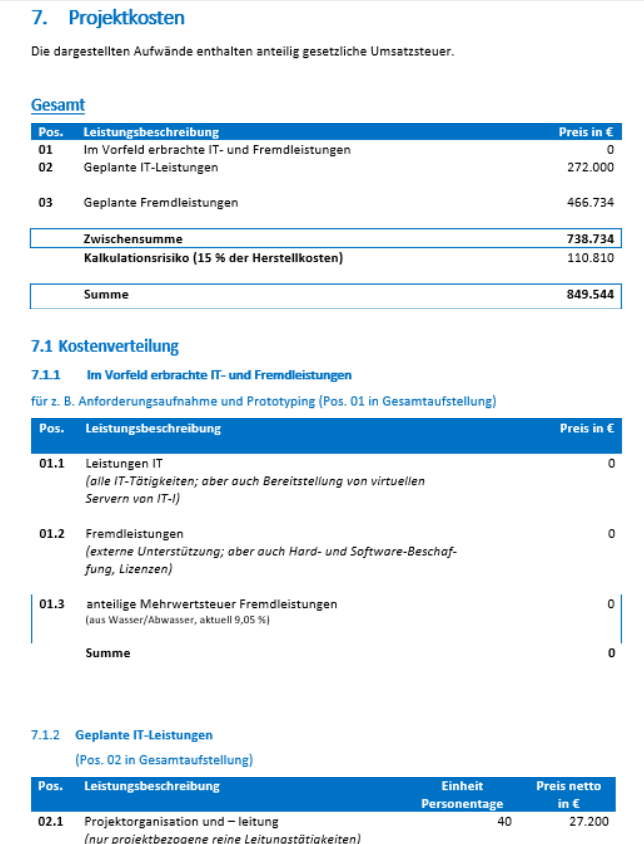
\includegraphics[width=1.0\textwidth]{BILDER-PTB4/kosten_1.png}
    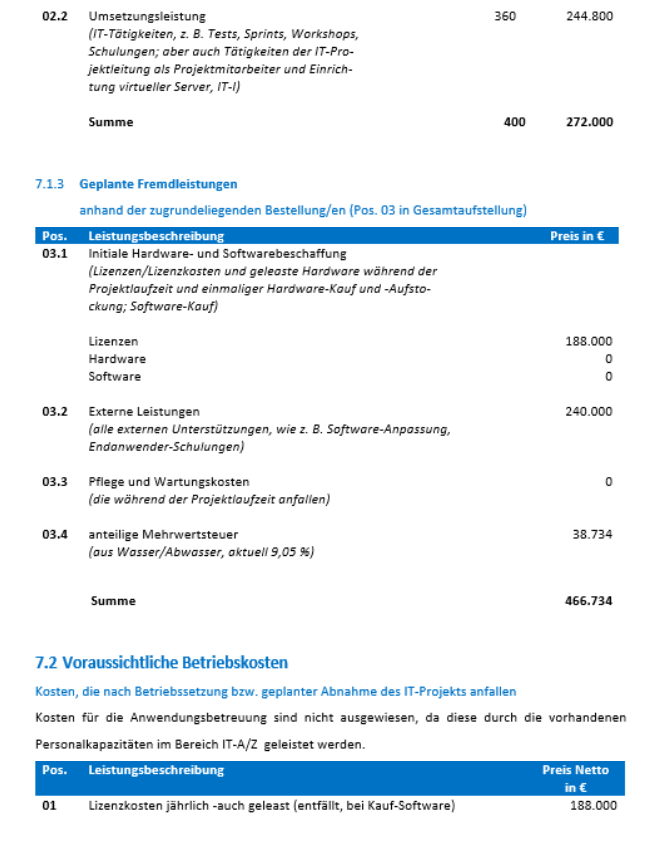
\includegraphics[width=1.0\textwidth]{BILDER-PTB4/kosten_2.png}
    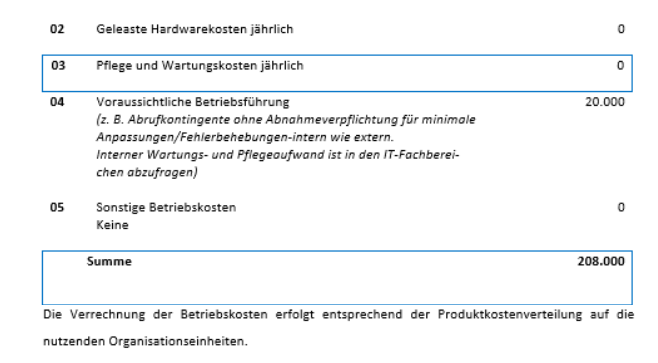
\includegraphics[width=1.0\textwidth]{BILDER-PTB4/kosten_3.png}
\end{center}

% Anhang 10
\newpage
\phantomsection
\addcontentsline{toc}{subsection}{Anhang 10: Kostencontrolling bei den BWB}
\label{sec:Anhang10}
\vspace*{\fill}
\begin{center}
    \begin{adjustbox}{rotate=90, center, valign=b}
        \begin{minipage}{0.95\textheight}
            \centering
            {\Large\bfseries Anhang 10: Kostencontrolling bei den BWB}\\[1em]
             {\normalsize Quelle: Eigene Darstellung in Anlehnung an die Kostencontrolling-Template bei den BWB}\\[0.4cm]
            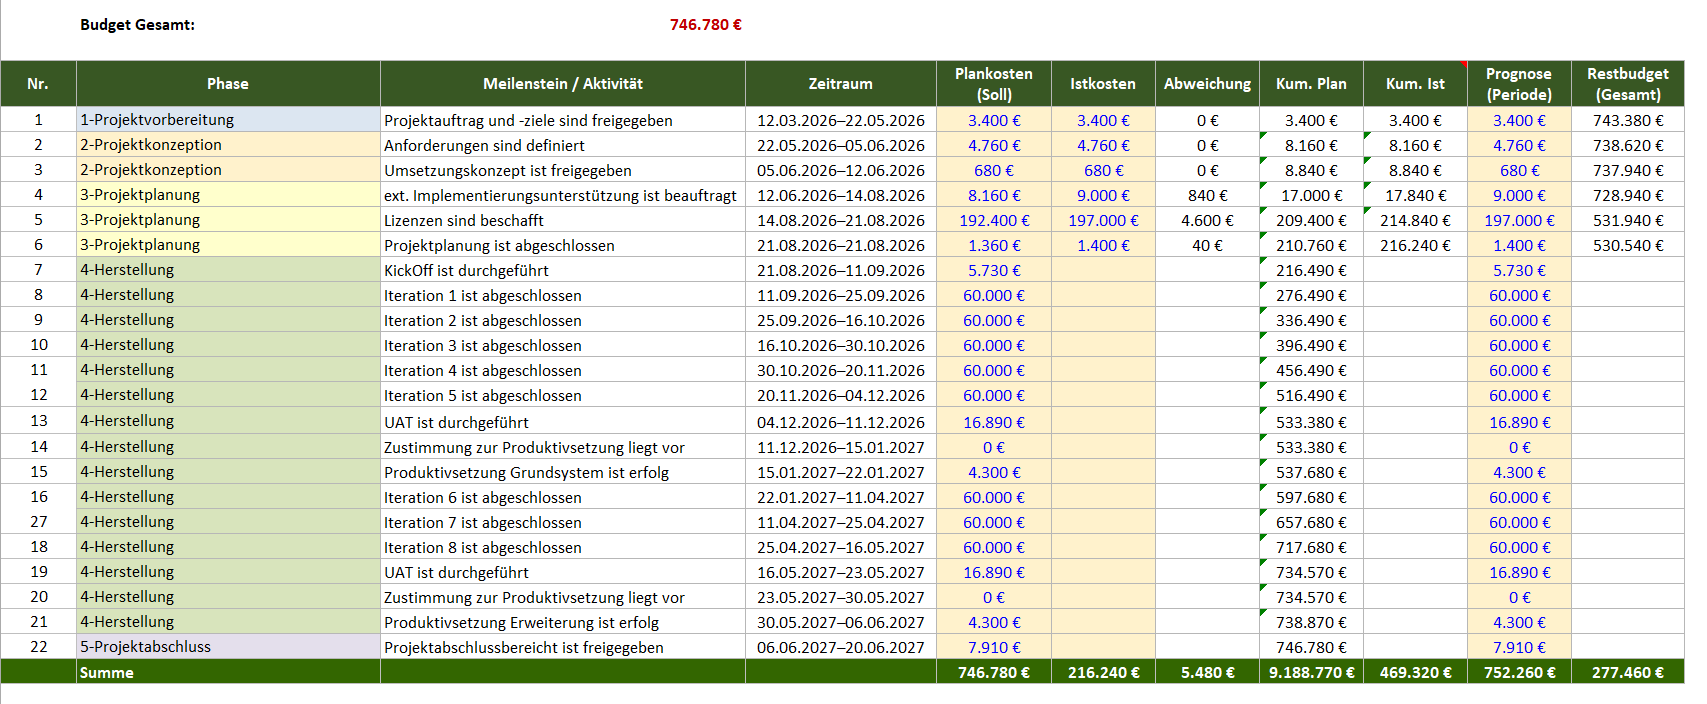
\includegraphics[width=0.9\textheight,keepaspectratio]{BILDER-PTB4/kostencontrolling_1.png}
             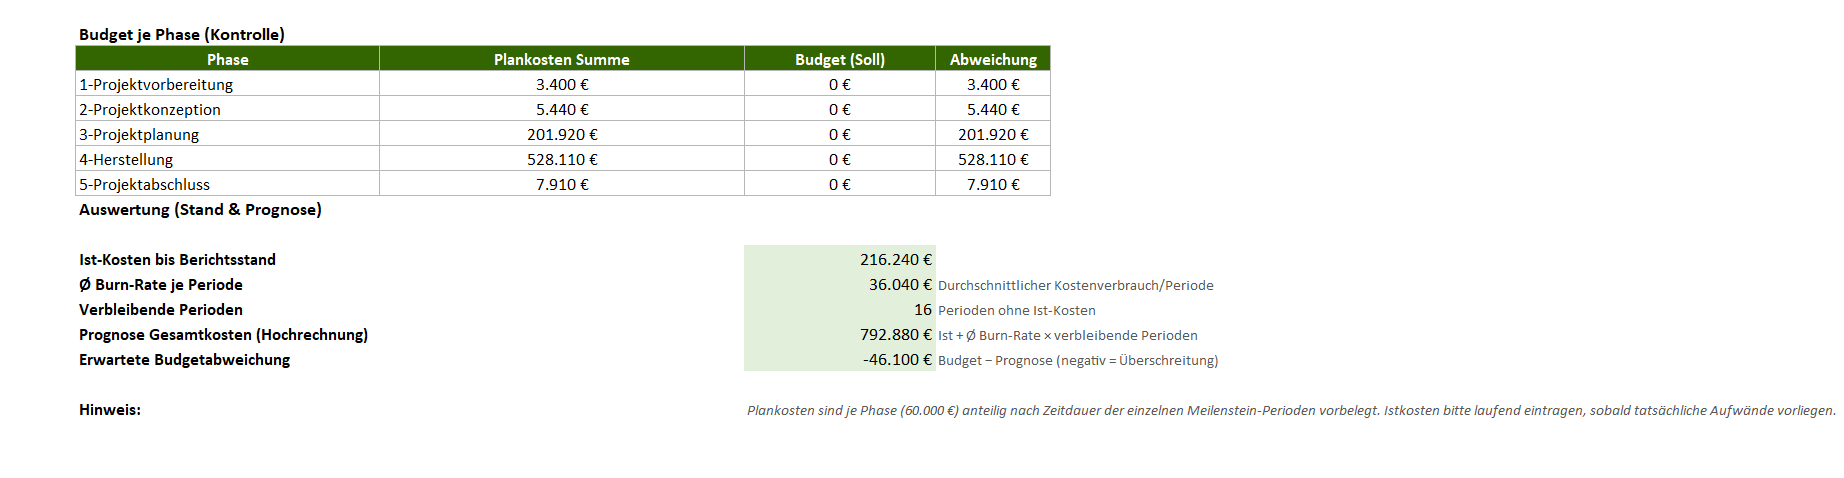
\includegraphics[width=1.0\textwidth]{BILDER-PTB4/kostencontrolling_2.png}
        \end{minipage}
    \end{adjustbox}
\end{center} 

% Anhang 11
\newpage
\phantomsection
\addcontentsline{toc}{subsection}{Anhang 11: Kostencontrolling Ist-Plankosten Grafik}
\label{sec:Anhang11}
\vspace*{\fill}
\begin{center}
    \begin{adjustbox}{rotate=90, center, valign=b}
        \begin{minipage}{0.95\textheight}
            \centering
            {\Large\bfseries Anhang 11: Kostencontrolling Ist-Plankosten Prognose - Grafik}\\[1em]
             {\normalsize Quelle: Eigene Darstellung in Anlehnung an die Projektkostensdokument bei den BWB}\\[0.4cm]
            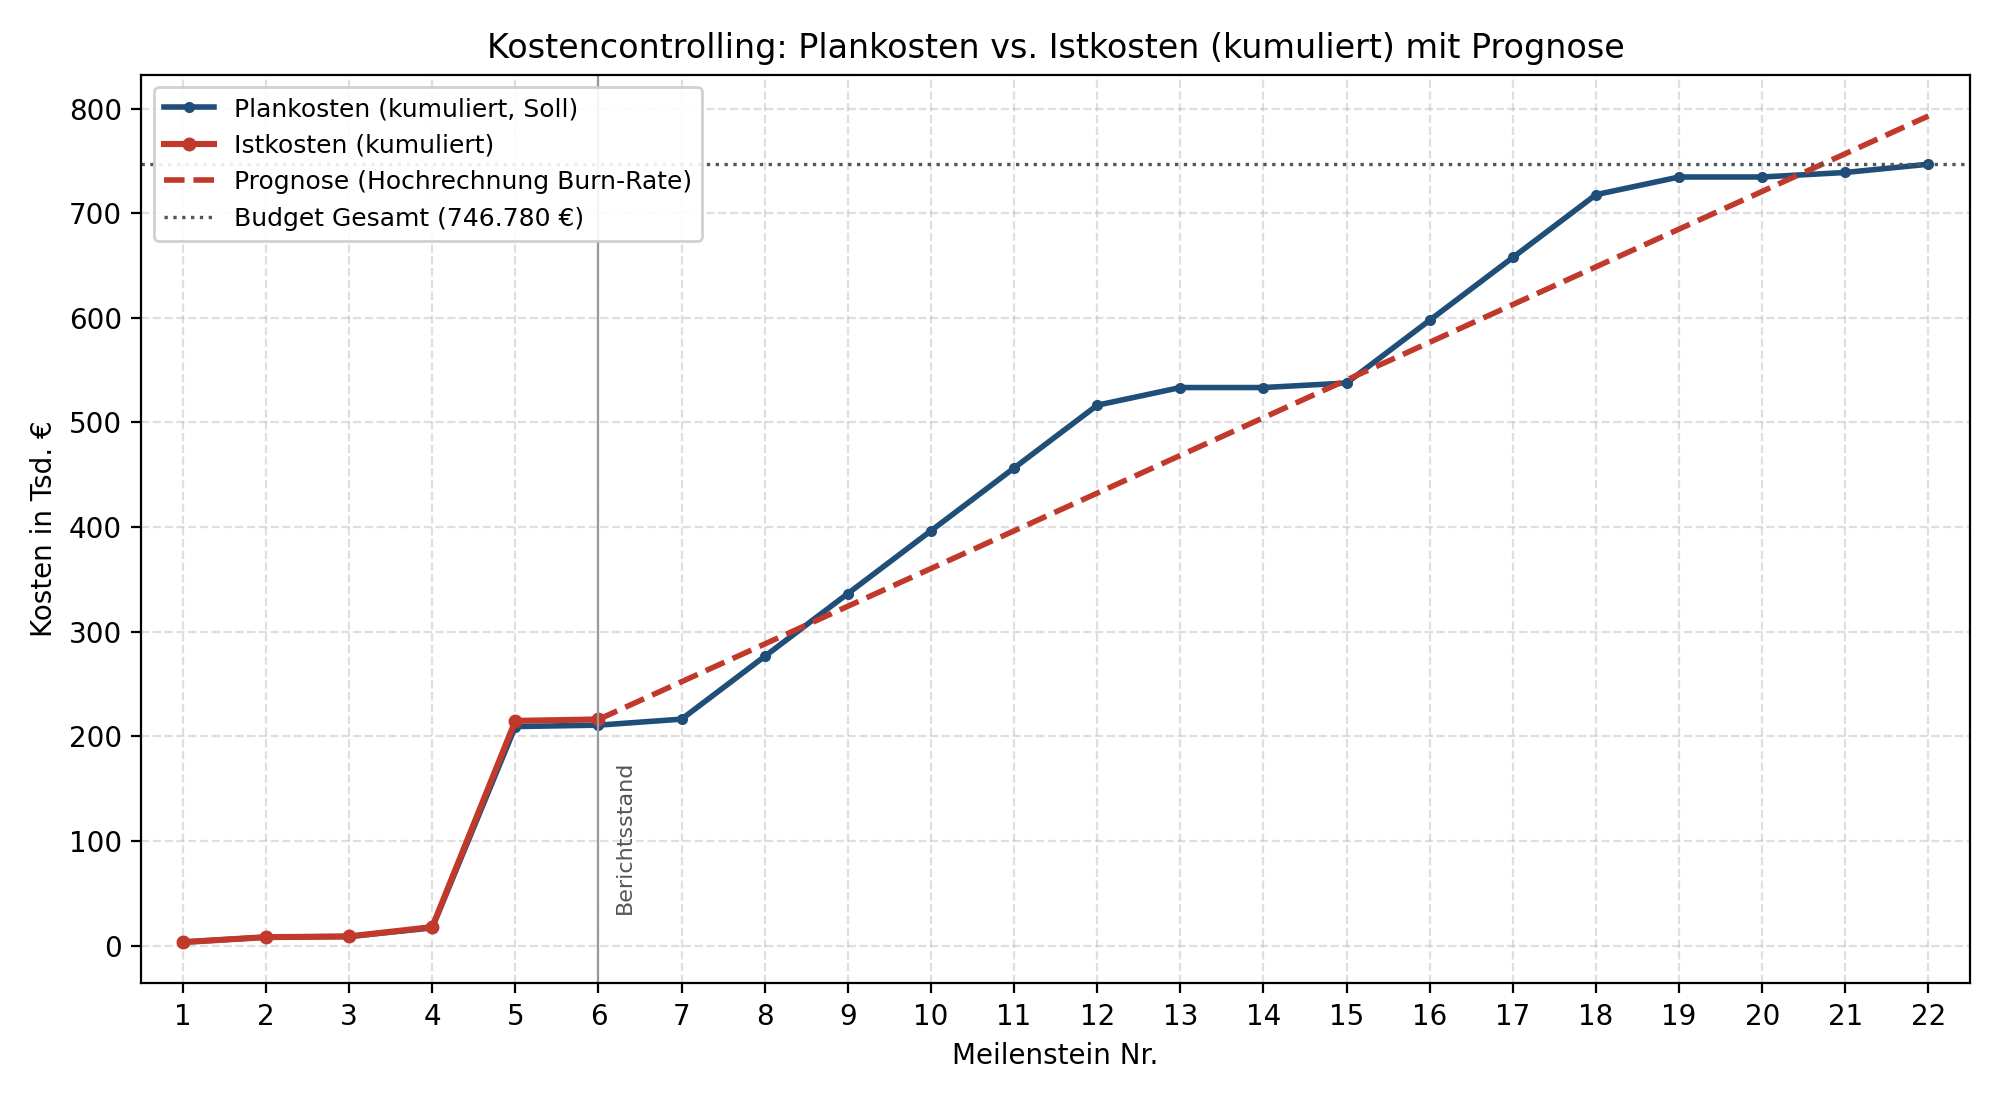
\includegraphics[width=0.9\textheight,keepaspectratio]{BILDER-PTB4/Kostencontrolling_Soll_Ist_Prognose.png}
        \end{minipage}
    \end{adjustbox}
\end{center} 

% Anhang 12
\newpage
\phantomsection
\addcontentsline{toc}{subsection}{Anhang 12: Leistungs-Qualitätscontrolling bei den BWB}
\label{sec:Anhang12}
\vspace*{\fill}
\begin{center}
    \begin{adjustbox}{rotate=90, center, valign=b}
        \begin{minipage}{0.95\textheight}
            \centering
            {\Large\bfseries Anhang 12: Leistungs-Qualitätscontrolling bei den BWB}\\[1em]
             {\normalsize Quelle: Eigene Darstellung in Anlehnung an die Projektkostensdokument bei den BWB}\\[0.4cm]
            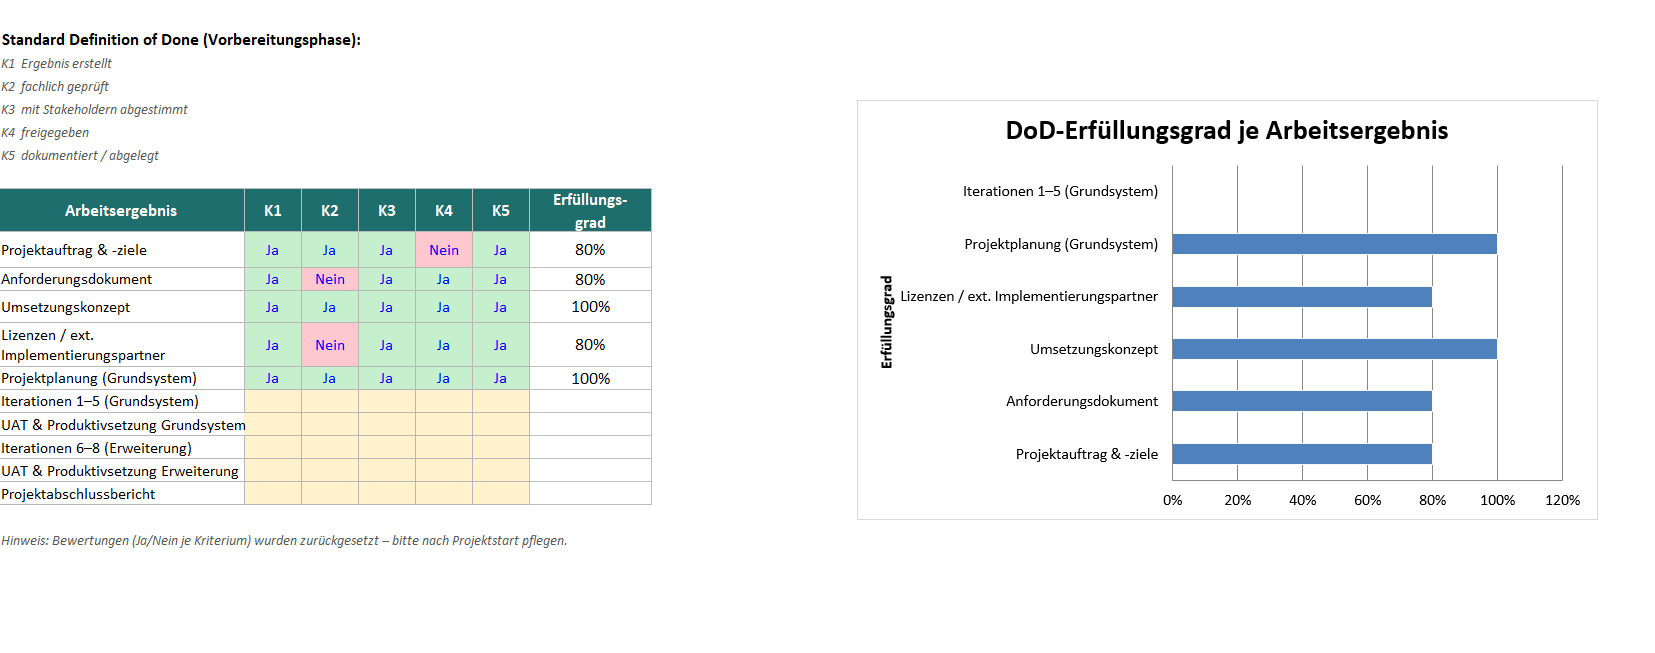
\includegraphics[width=0.9\textheight,keepaspectratio]{BILDER-PTB4/Leistungs-Qualitätscontrolling.png}
        \end{minipage}
    \end{adjustbox}
\end{center} 

% Anhang 13
\newpage
\phantomsection
\addcontentsline{toc}{subsection}{Anhang 13: Risikocontrolling bei den BWB}
\label{sec:Anhang13}
\vspace*{\fill}
\begin{center}
    \begin{adjustbox}{rotate=90, center, valign=b}
        \begin{minipage}{0.95\textheight}
            \centering
            {\Large\bfseries Anhang 13: Risikocontrolling bei den BWB}\\[1em]
             {\normalsize Quelle: Eigene Darstellung in Anlehnung an die Projektkostensdokument bei den BWB}\\[0.4cm]
            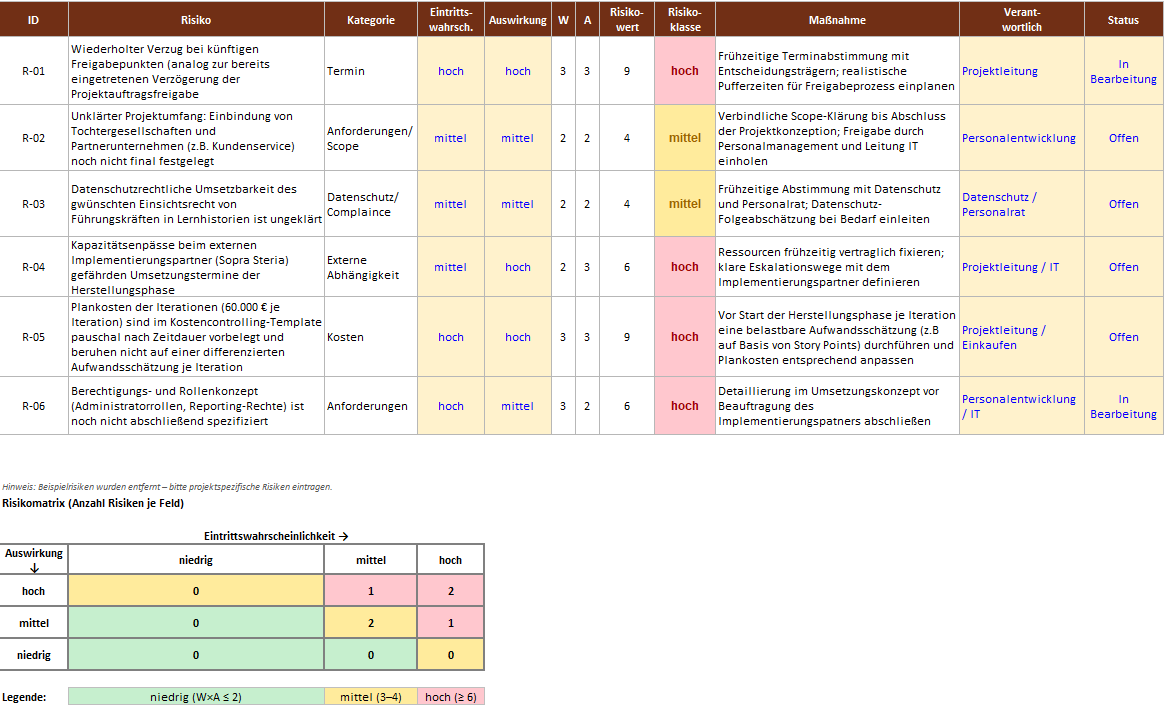
\includegraphics[width=0.9\textheight,keepaspectratio]{BILDER-PTB4/Risikocontrolling.png}
        \end{minipage}
    \end{adjustbox}
\end{center} 

%Anhang 14
\newpage
\phantomsection
\addcontentsline{toc}{subsection}{Anhang 14: Interviewprotokoll (Julia Steckler)}
\label{sec:Anhang14}

{\Large\bfseries Anhang 14: Interviewprotokoll}\\[1em]
\textbf{Interviewer:} Nicole Camille Bai\~ao \\
\textbf{Befragte:} Julia Steckler (Mitarbeiterin IT-Projektb\"uro) \\
\textbf{Datum:} 20. Juli 2026 \\
\textbf{Ort:} Berliner Wasserbetriebe, Neue J\"udenstra{\ss}e 1, 10179 Berlin

\bigskip
\noindent{\large\bfseries 1. Rolle und Aufgaben}

\textbf{Frage 1: Können Sie Ihre Rolle und Ihre Aufgaben kurz beschreiben?}

Julia: Ich bin im IT-Projektbüro bei IT-Z/P tätig, einer dauerhaften Instanz, die alle bei IT-Z/P betreuten IT-Projekte begleitet. Das IT-Projektbüro ist Anlaufstelle für IT-Projektleitungen bei Fragen, Problemen und Eskalationsthemen, übernimmt das On- und Offboarding interner sowie externer Mitarbeitender (u.\,a. Consultants, externe Projektleitungen) einschließlich Berechtigungsvergabe und führt regelmäßige Projektstatus-Meetings mit den Projektleitungen durch. Die Stelle war ursprünglich mit zwei Personen besetzt; seit dem Ausscheiden der Kollegin vor rund anderthalb Jahren wird die Aufgabe allein wahrgenommen.

\bigskip
\noindent{\large\bfseries 2. Aktuelles Vorgehen im Projektcontrolling}

\textbf{Frage 2: Wie wird der Projektstand aktuell erfasst und gesteuert?}

Julia: Der Projektstand wird in monatlichen Projektstatus-Meetings mit den jeweiligen IT-Projektleitungen erhoben. Erfasst werden u.\,a., ob das Projektportfolio und Stammblatt gepflegt sind, ob Ressourcen zugeordnet, ein grober Projektplan sowie Aktivitäten und Termine im Projektplanungstool Blue Ant hinterlegt und schlüssig sind, ob Zeiten gebucht wurden und ob der monatliche Statusbericht verschickt wurde. Die Ergebnisse werden zusätzlich in einer Excel-Tabelle mit Ampelsystem festgehalten, da Blue Ant aufgrund noch bestehender Einschränkungen kein vollständiges Reporting ermöglicht.

\textbf{Frage 3: Wie werden Termin- und Kostentreue konkret ermittelt?}

Julia: Termin- und Kostentreue werden nicht rechnerisch aus Meilensteinen oder Plan-/Ist-Werten in Blue Ant ermittelt, sondern nach Augenmaß anhand der Rücksprachen aus den Projektstatus-Meetings geschätzt. Am Monatsende werden alle Projekte gemeinsam mit dem Vorgesetzten (Projektleiter) anhand der Tabelle durchgegangen; dabei wird eingeschätzt, ob und wie stark sich Verzögerungen auf die zuletzt gemeldete Termintreue auswirken (z.\,B. Abwertung von 86 auf 80\,Prozent bei erkennbaren Risiken). Die so festgelegte Termin- und Kostentreue wird anschließend per E-Mail an die Bereichsleitung IT gemeldet.

\textbf{Frage 4: Nach welchen Schwellenwerten funktioniert das Ampelsystem?}

Julia: Werte zwischen 80 und 100\,Prozent gelten als grün, Werte zwischen 70 und 79\,Prozent als gelb, Werte unter 70\,Prozent als rot.

\bigskip
\noindent{\large\bfseries 3. Vorgehen vor Einführung von Blue Ant}

\textbf{Frage 5: Wie wurde der Projektstand vor Einführung von Blue Ant erfasst?}

Julia: Zuvor wurden Kosten- und Termintreue in zwei getrennten Excel-Dateien geführt. Für die Kostentreue wurden je Projekt Angebotswert (Planwert), Ist-Kosten und voraussichtliche Ist-Kosten erfasst, die ebenfalls aus den Projektstatus-Meetings mit den IT-Projektleitungen stammten; daraus ließen sich Unter- oder Überschreitungen gegenüber dem Planwert ablesen. Diese Vorgehensweise wird aktuell nicht mehr angewendet.

\bigskip
\noindent{\large\bfseries 4. Qualitätscontrolling}

\textbf{Frage 6: Wie wird die Qualität eines Projekts bzw. der entwickelten Software kontrolliert?}

Julia: Ein eigenständiges Instrument zur Qualitätskontrolle existiert nicht; die Einschätzung der Qualität ergibt sich aus der laufenden Begleitung der Projekte. Das IT-Projektbüro ist im Regelfall bereits ab der ersten Projektphase eingebunden, in der Auftrag und Ziel des Projekts festgelegt werden, und erhält über die monatlichen Projektstatus-Meetings kontinuierlich Einblick in den fachlichen und technischen Fortschritt. Werden dabei unklare oder unrealistische Anforderungen erkennbar, wird der Projektleitung empfohlen, Rücksprache mit dem Fachbereich bzw. Auftraggeber zu halten.

\bigskip
\noindent{\large\bfseries 5. Herausforderungen und geplante Weiterentwicklung}

\textbf{Frage 7: Welche Herausforderungen bestehen aktuell im Projektcontrolling?}

Julia: Durch den Weggang der Kollegin wird die Aufgabe seit rund anderthalb Jahren allein wahrgenommen, wodurch die geplante Weiterentwicklung der KPIs sowie die vollständige Ablösung der Excel-Lösung durch Blue Ant zunehmend nachrangig priorisiert wurden. Blue Ant kann derzeit noch nicht vollumfänglich genutzt werden, sodass ein manueller Parallelbetrieb mit Excel-Tabellen erforderlich bleibt. Zusätzlicher Aufwand entstand durch die Neuerfassung und laufende Überarbeitung projektphasenbezogener Dokumente (Phasenoutputs) sowie zugehöriger Prozessanpassungen.

\textbf{Frage 8: Ist eine Rückkehr zu einer rechnerisch ermittelten Termin- und Kostentreue geplant?}

Julia: Ziel ist es, wieder zu einer rechnerisch ermittelten statt einer geschätzten Termintreue zurückzukehren, sobald die Rahmenbedingungen (u.\,a. Personalsituation, vollständige Nutzbarkeit von Blue Ant) dies zulassen.

% Anhang 15
\newpage
\phantomsection
\addcontentsline{toc}{subsection}{Anhang 15: Projektcontrolling - Excel-Tabelle}
\label{sec:Anhang15}
\vspace*{\fill}
\begin{center}
    \begin{adjustbox}{rotate=90, center, valign=b}
        \begin{minipage}{0.95\textheight}
            \centering
            {\Large\bfseries Anhang 15: Projektcontrolling - Excel-Tabelle}\\[1em]
             {\normalsize interne Quelle: Besipiel von Projektcontrolling - Excel-Tabelle bei den BWB}\\[0.4cm]
            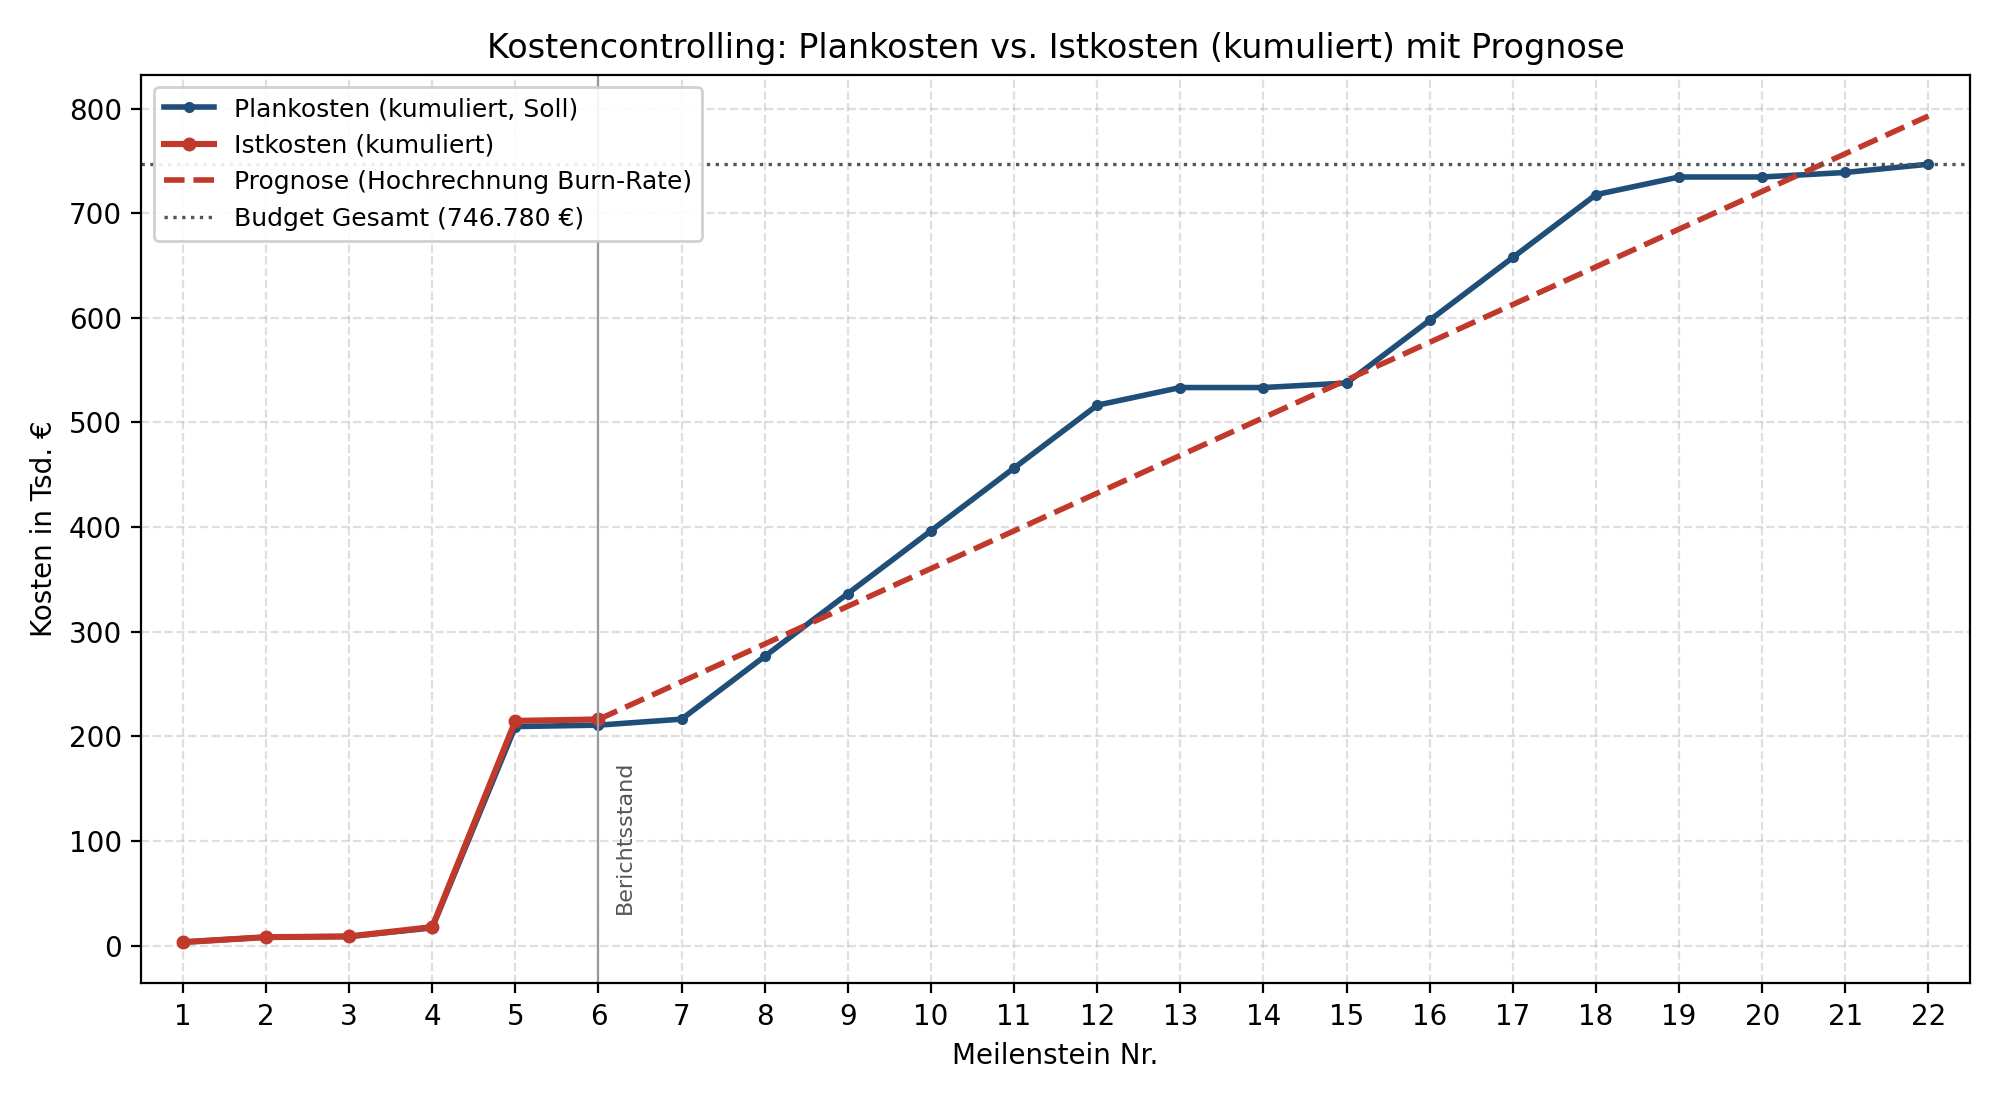
\includegraphics[width=0.9\textheight,keepaspectratio]{BILDER-PTB4/Kostencontrolling_Soll_Ist_Prognose.png}
        \end{minipage}
    \end{adjustbox}
\end{center} 

% Anhang 16
\newpage
\phantomsection
\addcontentsline{toc}{subsection}{Anhang 16: KI-Verzeichnis}
\label{sec:Anhang16}

{\Large\bfseries Anhang 16: KI-Verzeichnis}\\[0.6cm]

\begin{tabular}{|p{3.2cm}|p{5.2cm}|p{4.2cm}|p{3.2cm}|}
    \hline
    \textbf{KI-basiertes Hilfsmittel} & \textbf{Einsatzform} & \textbf{Betroffene Teile der Arbeit} & \textbf{Bemerkungen} \\
    \hline
    ChatGPT (OpenAI) & Verbesserung der Textformulierung und Grammatik. & Ganze Arbeit. & Nur Sprachkorrektur, keine inhaltliche Änderung. \\
    \hline
    DeepL Translator & Übersetzung von Textpassagen. & Ganze Arbeit. & Übersetzung einzelner Wörter sowie kurzer Sätze. \\
    \hline
\end{tabular}

% === Ehrenwörtliche Erklärung ===
\newpage
\section*{Ehrenwörtliche Erklärung}
\phantomsection
\addcontentsline{toc}{section}{Ehrenwörtliche Erklärung}

„Ich erkläre ehrenwörtlich:

dass ich die vorliegende Arbeit in allen Teilen selbstständig angefertigt und keine anderen als
die in der Arbeit angegebenen Quellen und Hilfsmittel benutzt habe, und dass die Arbeit in
gleicher oder ähnlicher Form in noch keiner anderen Prüfung vorgelegen hat. Sämtliche wörtlichen oder sinngemäßen Übernahmen und Zitate, sowie alle Abschnitte, die mithilfe von KI-basierten Tools entworfen, verfasst und/oder bearbeitet wurden, sind kenntlich gemacht und
nachgewiesen. Im Anhang meiner Arbeit habe ich sämtliche KI-basierte Hilfsmittel angegeben.
Diese sind mit Produktnamen und formulierten Eingaben (Prompts) in einem KI-Verzeichnis
ausgewiesen.

Ich bin mir bewusst, dass die Verwendung von Texten oder anderen Inhalten und Produkten, die durch KI-basierte Tools generiert wurden, keine Garantie für deren Qualität darstellt. Ich verantworte die Übernahme jeglicher von mir verwendeter maschinell generierter Passagen vollumfänglich selbst und trage die Verantwortung für eventuell durch die KI
generierte fehlerhafte oder verzerrte Inhalte, fehlerhafte Referenzen, Verstöße gegen das
Datenschutz- und Urheberrecht oder Plagiate.
% --- Tabelle mit Unterschriften ---

\begin{tabular}{p{8cm}}
    \normalsize{Berlin, den 02. März 2026.} \\[0.5cm]
    
\includegraphics[width=5.5cm]{BILDER-PTB4/unterschrift_nicole.png} \\
    \normalsize{\underline{\hspace{5.5cm}}} \\
    \normalsize{(Unterschrift der Studentin)}
\end{tabular} % \underline{\hspace{6cm}} erzeugt eine Linie mit einer Länge von 6 cm


% === ENDE DOKUMENT ===
\end{document}
